\documentclass[../main.tex]{subfiles}
\begin{document}
%\chapter{Results}\label{ch:A}
In this chapter will focus on the effects on the performance of quantum annealing algorithm upon adding the second trigger, namely the anti-ferromagnetic trigger, to the original Hamiltonian. Unlike in the case of the ferromagnetic trigger, for anti-ferromagnetic trigger the strength parameter, g in Eq. (\ref{eq:b12}) plays a more decisive role than merely controlling the extent by which the minimum gap is enlarged. The anti-ferromagnetic trigger alters the energy spectra, the minimum energy gaps, and the number of anti-crossings between the ground and first excited energy state of the Hamiltonian, depending on the strength with which the trigger is added, as well as on the problem itself. We shall begin by observing the effects of adding the anti-ferromagnetic trigger to the original Hamiltonian, for the three chosen problems. The following sections will then showcase the role that the strength parameter - g plays.

\section*{The chosen problems}
Let us begin by considering problem 733 again, which was found to have large success probability for the original Ising Hamiltonian in the problem. \\
Figs. (\ref{fig:a1}), (\ref{fig:a2}) and (\ref{fig:a3}) show the energy spectra and the energy expectation values for the instantaneous state corresponding to the three annealing times, after adding the anti-ferromagnetic trigger to the Hamiltonian with strengths 0.5, 1 and 2 respectively.
\begin{figure}[H]
\centering 
\includegraphics[scale=0.24]{733_s12_A_g0.png}
\caption{The energy spectrum and energy expectation values for the instantaneous state of problem 733, after adding the anti-ferromagnetic trigger with g=0.5, for the three annealing times. $\Delta_{min}$ was found to be 0.3070, while $p$=0.9117 for $T_A$=100. }
\label{fig:a1}
\end{figure}
\begin{figure}[H]
\centering 
\includegraphics[scale=0.24]{733_s12_A_g1.png}
\caption{The energy spectrum and energy expectation values for the instantaneous state of problem 733, after adding the anti-ferromagnetic trigger with g=1, for the three annealing times. $\Delta_{min}$ was found to be 0.1349, while $p$=0.5747 for $T_A$=100. }
\label{fig:a2}
\end{figure}
\begin{figure}[H]
\centering 
\includegraphics[scale=0.24]{733_s12_A_g2.png}
\caption{The energy spectrum and energy expectation values for the instantaneous state of problem 733, after adding the anti-ferromagnetic trigger with g=2, for the three annealing times. $\Delta_{min}$ was found to be 0.0020, while $p$=0.0273 for $T_A$=100. }
\label{fig:a3}
\end{figure}
Tab. (\ref{tab:a1}) shows a comparison of the success probabilities - p, and minimum energy gaps - $\Delta_{min}$ between the original Hamiltonian and the Hamiltonian after adding the anti-ferromagnetic triggers with different strengths for problem 733.

\begin{table}[H]
\centering
\renewcommand{\arraystretch}{1.5}
\begin{tabular}{|c|c|c|c|c|}
\hline 
Problem 733 & Original Hamiltonian & Trigger=A, g=0.5 & Trigger=A, g=1 & Trigger=A, g=2 \\ 
\hline 
$\Delta_{min}$ & 0.4407 & 0.3070 & 0.1349 & 0.0020 \\ 
\hline 
p($T_A$=10) & 0.3444 & 0.1446 & 0.0279 & 1.271 $\times 10^{-4}$ \\ 
\hline 
p($T_A$=100) & 0.9944 & 0.9117 & 0.5747 & 0.0273 \\ 
\hline 
p($T_A$=1000) & 0.9999 & 0.9999 & 0.9999 & 0.8761 \\ 
\hline 
s value at $\Delta_{min}$ & 0.459 & 0.367 & 0.282 & 0.254 \\ 
\hline
Number of anti-crossings & 1 & 2 & 1 & 4 \\
\hline
\end{tabular} 
\caption{A comparison of the minimum energy gaps and the success probabilities for problem 733, between the original Hamiltonian and the Hamiltonian with anti-ferromagnetic trigger (A) of different strengths. The minimum gaps become successively smaller as the strength of the anti-ferromagnetic trigger is increased. The success probabilities are decreased as a result. The value of s corresponding to the position of the minimum gap also becomes smaller.}
\label{tab:a1}
\end{table}
As can be noted from the table above, the minimum energy gap decreases upon adding the ferromagnetic trigger, and this decrease becomes larger as the strength of the trigger is increased. Consequently, the success probabilities after adding the trigger are found to be decreasing as well. The value of annealing parameter - s also becomes smaller with increasing strength of the trigger.\\
Additionally, a different feature that was observed as a result of adding the anti-ferromagnetic trigger (compared to the effects of adding the ferromagnetic trigger) was the change in the number of anti-crossings between the ground and the first energy state. For strengths g=0.5 and g=2, the number of energy anti-crossings increased to 2 and 4 respectively, while for g=1 it remained unchanged. Moreover, when the anti-ferromagnetic trigger is added with strength 2, the energy spectrum changed significantly (in terms of the number of the energy anti-crossings between the energy levels of the spectrum and the width of the anti-crossing) in comparison to the original spectrum (see Fig. \ref{fig:o2}), as can be more clearly seen in the inset of Fig. (\ref{fig:a3}).\\

Next, let us consider problem 950 that had small success probability in absence of any triggers. Figs. (\ref{fig:a4}), (\ref{fig:a5}), and (\ref{fig:a6}) show the energy spectrum and the energy expectation values for the instantaneous state corresponding to the three annealing times, after adding the anti-ferromagnetic trigger to the Hamiltonian with strengths 0.5, 1 and 2 respectively. 


\begin{figure}[H]
\centering 
\includegraphics[scale=0.24]{950_s12_A_g0.png}
\caption{The energy spectrum and energy expectation values for the instantaneous state of problem 950, after adding the anti-ferromagnetic trigger with g=0.5, for the three annealing times. $\Delta_{min}$ was found to be 0.0130, while $p$=0.0022 for $T_A$=100. }
\label{fig:a4}
\end{figure}
\begin{figure}[H]
\centering 
\includegraphics[scale=0.24]{950_s12_A_g1.png}
\caption{The energy spectrum and energy expectation values for the instantaneous state of problem 950, after adding the anti-ferromagnetic trigger with g=1, for the three annealing times. $\Delta_{min}$ was found to be 0.0019, while $p$=0.0239 for $T_A$=100. }
\label{fig:a5}
\end{figure}
\begin{figure}[H]
\centering 
\includegraphics[scale=0.24]{950_s12_A_g2.png}
\caption{The energy spectrum and energy expectation values for the instantaneous state of problem 950, after adding the anti-ferromagnetic trigger with g=2, for the three annealing times. $\Delta_{min}$ was found to be 0.1784, while $p$=0.4468 for $T_A$=100. }
\label{fig:a6}
\end{figure}
For this case, Tab. (\ref{tab:a2}) shows a comparison of the minimum energy gaps, and success probabilities (corresponding to different annealing times) between the original Hamiltonian and the Hamiltonian upon adding the anti-ferromagnetic trigger with different strengths. 

\begin{table}[H]
\centering
\renewcommand{\arraystretch}{1.5}
\begin{tabular}{|c|c|c|c|c|}
\hline 
Problem 950 & Original Hamiltonian & Trigger=A, g=0.5 & Trigger=A, g=1 & Trigger=A, g=2 \\ 
\hline 
$\Delta_{min}$ & 0.0312 & 0.0130 & 0.0019 & 0.1784 \\ 
\hline 
p($T_A$=10) & 2.343 $\times 10^{-4}$ & 0.0567 & 0.0017 & 0.0071\\ 
\hline 
p($T_A$=100) & 0.0146 & 0.0022 & 0.0239 & 0.4468 \\ 
\hline 
p($T_A$=1000) & 0.1362 & 0.0228 & 0.1729 & 0.9999 \\ 
\hline 
s value at $\Delta_{min}$ & 0.665 & 0.644 & 0.601 & 0.263 \\ 
\hline 
Number of anti-crossings & 1 & 1 & 2 & 3 \\
\hline
\end{tabular} 
\caption{A comparison of the minimum gaps and the success probabilities for problem 950, between the original Hamiltonian and the Hamiltonian with anti-ferromagnetic trigger (A) of different strengths. The minimum gap becomes small for g=0.5, and even smaller for g=1, while it becomes even larger than the original minimum energy gap for g=2. The value of s corresponding to the position of the minimum gap becomes smaller with increasing strength of the trigger.}
\label{tab:a2}
\end{table}


The minimum energy gaps decrease with respect to the original minimum gaps, upon adding the trigger with strengths 0.5, and 1. However, the success probability for $T_A$=10 after adding the anti-ferromagnetic trigger with g=0.5 and g=1, is larger compared to that of the original Hamiltonian, owing to different reasons.\\

Since upon adding the anti-ferromagnetic trigger with strength 0.5, the minimum energy gap becomes smaller, the annealing time of $T_A$=10 is so short that the state of the system transits to the first excited state even before the minimum gap anti-crossing. Upon approaching the minimum gap anti-crossing the system state shifts some of the amplitude back to the ground state, increasing the success probability in this case (see Fig. \ref{fig:a4}). However, for the original Hamiltonian the gap is not large enough for an annealing time of 10 for the state to shift to the first excited state before the minimum energy gap (see Fig. \ref{fig:o3}). The state therefore stays close to the first excited state after passing the anti-crossing.\\
Furthermore, for annealing times $T_A$=100 and $T_A$=1000, the system state transitions only at the minimum gap anti-crossing and closely follows the second and first excited states respectively. The overlap with the ground state decreases, and therefore the success probability in both these cases also reduces.\\

In the case of adding the anti-ferromagnetic trigger with strength 1, the number of energy anti-crossings increases to 2. The first energy anti-crossing is small enough for just $T_A$=10 to shift the system state to the first excited state. Quickly after transitioning to the first excited state, the system state shifts to higher energy levels (Fig. \ref{fig:a5}). Since the state of the system is a superposition of many energy eigenstates, the present state of system has small, yet finite overlap with the ground state. In the original Hamiltonian, however, the system state shifts to the first excited state at the only energy anti-crossing, and therefore the overlap with the ground state becomes negligible (figure \ref{fig:o3}).\\

By choosing the strength to be 2, the minimum energy gap for this problem becomes larger than the original minimum energy gap, while the number of anti-crossings between the ground and the first excited state increases to 3. The success probability in this case is always larger than the original success probability for all annealing times. For $T_A$=10, the state of the system shifts to the first excited state at first energy anti-crossing, and then quickly shifts to a superposition state with the higher energy states (due to the proximity of the higher energy levels as result of adding the trigger). This results in a larger overlap with the ground state compared to the case of the state closely following the first excited state after reaching the only energy anti-crossing in case of the original problem (see Fig. \ref{fig:o3}).

For $T_A$=100, the state starts transitioning to the first excited state only as it approaches the second energy anti-crossing. The state does further shift to higher energy levels, but comes back to the first excited state before the third energy anti-crossing. At the third anti-crossing some of the amplitude of the wave function shifts to the ground state again, and therefore the success becomes larger than the original problem. 


Finally, for $T_A$=1000, the annealing time and the minimum energy gap is large enough for the system to always stay close to the ground state, hence the larger success probability.\\

Lastly, figures (\ref{fig:a7}), (\ref{fig:a8}) and (\ref{fig:a9}) show the energy spectra and the energy expectation values for the state for problem 528, after adding the anti-ferromagnetic trigger with strengths 0.5, 1 and 2 respectively. 


\begin{figure}[H]
\centering 
\includegraphics[scale=0.24]{528_s12_A_g0.png}
\caption{The energy spectrum and energy expectation values for the instantaneous state of problem 528, after adding the anti-ferromagnetic trigger with g=0.5, for the three annealing times. $\Delta_{min}$ was found to be 0.0049, while $p$=0.0120 for $T_A$=100. }
\label{fig:a7}
\end{figure}
\begin{figure}[H]
\centering 
\includegraphics[scale=0.24]{528_s12_A_g1.png}
\caption{The energy spectrum and energy expectation values for the instantaneous state of problem 528, after adding the anti-ferromagnetic trigger with g=1, for the three annealing times. $\Delta_{min}$ was found to be 0.0562, while $p$=0.1517 for $T_A$=100. }
\label{fig:a8}
\end{figure}
\begin{figure}[H]
\centering 
\includegraphics[scale=0.24]{528_s12_A_g2.png}
\caption{The energy spectrum and energy expectation values for the instantaneous state of problem 528, after adding the anti-ferromagnetic trigger with g=2, for the three annealing times. $\Delta_{min}$ was found to be 0.1008, while $p$=0.0480 for $T_A$=100. }
\label{fig:a9}
\end{figure}

Tab. (\ref{tab:a3}) shows a comparison of the minimum energy gaps, and success probabilities (corresponding to different annealing times) between the original Hamiltonian and the Hamiltonian upon adding the anti-ferromagnetic trigger with different strengths for problem 528. 

\begin{table}[H]
\centering
\renewcommand{\arraystretch}{1.5}
\begin{tabular}{|c|c|c|c|c|}
\hline 
Problem 528 & Original Hamiltonian & Trigger=A, g=0.5 & Trigger=A, g=1 & Trigger=A, g=2 \\ 
\hline 
$\Delta_{min}$ & 0.1573 & 0.0049 & 0.0562 & 0.1008 \\ 
\hline 
p($T_A$=10) & 0.1577 & 0.0573 & 0.0368 & 4.21 $\times 10^{-5}$\\ 
\hline 
p($T_A$=100) & 0.5199 & 0.0120 & 0.1517 & 0.0480 \\ 
\hline 
p($T_A$=1000) & 0.9992 & 0.0071 & 0.6565 & 0.9313 \\ 
\hline 
s value at $\Delta_{min}$ & 0.514 & 0.454 & 0.418 & 0.256 \\ 
\hline 
Number of anti-crossings & 1 & 1 & 3 & 4 \\
\hline
\end{tabular} 
\caption{A comparison of the minimum energy gaps and the success probabilities for problem 528, between the original Hamiltonian and and the Hamiltonian with anti-ferromagnetic trigger (A) of different strengths. The minimum energy gaps after adding the trigger are smaller than the original minimum gap, for all the values of g. They however become large upon increasing the strength of the anti-ferromagnetic trigger. The value of s corresponding to the position of the minimum gap becomes smaller with increasing strength of the trigger.}
\label{tab:a3}
\end{table}

For this problem, it was observed that adding the anti-ferromagnetic trigger made the minimum energy gaps smaller than the original gap, for all the three values of the strength chosen. The gaps however increased with increasing the strength of the trigger. The original success probabilities, for all annealing times, are therefore larger than the resulting success probabilities upon adding the triggers with different g. Additionally, for all the annealing times but $T_A$=10, the success probabilities become larger when the anti-ferromagnetic trigger is added with strength 1 compared to when added with strength 0.5, as the minimum energy gap for the former is larger. For $T_A$=10, and both g=0.5 and g=1 cases, the system state transitions to the first excited state prior to the first energy anti-crossing. This is followed by the state shifting to higher energy levels soon after. Since the energy spectrum becomes more complex (in terms of the number of anti-crossings between the higher energy states and their proximity) as the strength of the trigger is increased, the system state shifts farther away from the ground state. Coincidentally, the state of the system with g=0.5 ends in a superposition state with a higher overlap with the ground state than the final state of the system with g=1.

 Although the gap becomes even larger with g=2, the success probability in this case is smaller compared to the case with g=1 for $T_A$=10 and $T_A$-1000. This can be explained by observing that adding the anti-ferromagnetic trigger with g=2 changes the energy spectrum of the Hamiltonian even more drastically. Not only do the number of energy anti-crossings between the ground and the first excited state increase to 4, the higher lying energy levels also become more involved and have larger number of crossings and anti-crossings. Therefore, as annealing times $T_A$=10 and $T_A$=100 are not large enough for the state to stay close to the ground state upon reaching the first energy anti-crossing, the system state settles even farther away from the ground state as compared to the g=1 case. The overlap of the  resulting state with the ground state is even smaller and hence, the success probability for $T_A$=10 and g=2 case is negligible. As the annealing time is increased further to $T_A$=1000, the minimum energy gap becomes large enough to keep the state of the system close to the ground state, and the success probability becomes comparable to the original success probability.
 
 
\section*{g=0.5}
This section will showcase the effects of adding the anti-ferromagnetic trigger to  all the original Hamiltonians from the set of 12 spin problems, with strength 0.5. For each problem, annealing time was chosen to be 10, 100 and 1000. 

As a measure of quantifying the performance with respect to the original Hamiltonian, relative success probability was defined as the ratio of the success probability upon adding the anti-ferromagnetic trigger ($p^A$) to the original success probability ($p^O$). Figs. (\ref{fig:a10}), (\ref{fig:a11}) and (\ref{fig:a12}) show the  distribution of the relative success probability for annealing times of 10, 100 and 1000 respectively, with the strength of the trigger Hamiltonian chosen to be 0.5.

\begin{figure}[H]
\centering 
\includegraphics[scale=0.24]{A_T10_g0.png}
\caption{Distribution of the relative success probability $\dfrac{p^A}{p^O}$ for g=0.5 and $T_A$=10. 43.9\% of the cases were found to have a higher success probability after adding the trigger.}
\label{fig:a10}
\end{figure}
\begin{figure}[H]
\centering 
\includegraphics[scale=0.24]{A_T100_g0.png}
\caption{Distribution of the relative success probability $\dfrac{p^A}{p^O}$ for $T_A$=100. 0.2\% of the cases were found to have a higher success probability after adding the trigger. }
\label{fig:a11}
\end{figure}
\begin{figure}[H]
\centering 
\includegraphics[scale=0.24]{A_T1000_g0.png}
\caption{Distribution of the relative success probability $\dfrac{p^A}{p^O}$ for $T_A$=1000. 0.2\% of the cases were found to have a higher success probability after adding the trigger.}
\label{fig:a12}
\end{figure}

For an annealing time $T_A$=10, it was found that 43.9\% of the problems of the set were improved after including the anti-ferromagnetic trigger with g=0.5. On increasing the annealing time to 100 and 1000, the percentage of cases with improved success probability dropped to 0.2\% for both the cases. Furthermore, the largest value of the relative success ratio is a little more than 250 for $T_A$=10, while it reduces to 1.995 for $T_A$=100, and to 1.585 for $T_A$=1000. In order to understand the reasons for this decrease in the relative success ratio on increasing the annealing time, the minimum energy gaps of all the problems were calculated after adding the trigger. Fig. (\ref{fig:a13}) shows a plot of the minimum energy gaps after adding the anti-ferromagnetic trigger ($\Delta_{min}^A$) with the original minimum energy gaps ($\Delta_{min}^O$) with g=0.5.
\begin{figure}[H]
\centering 
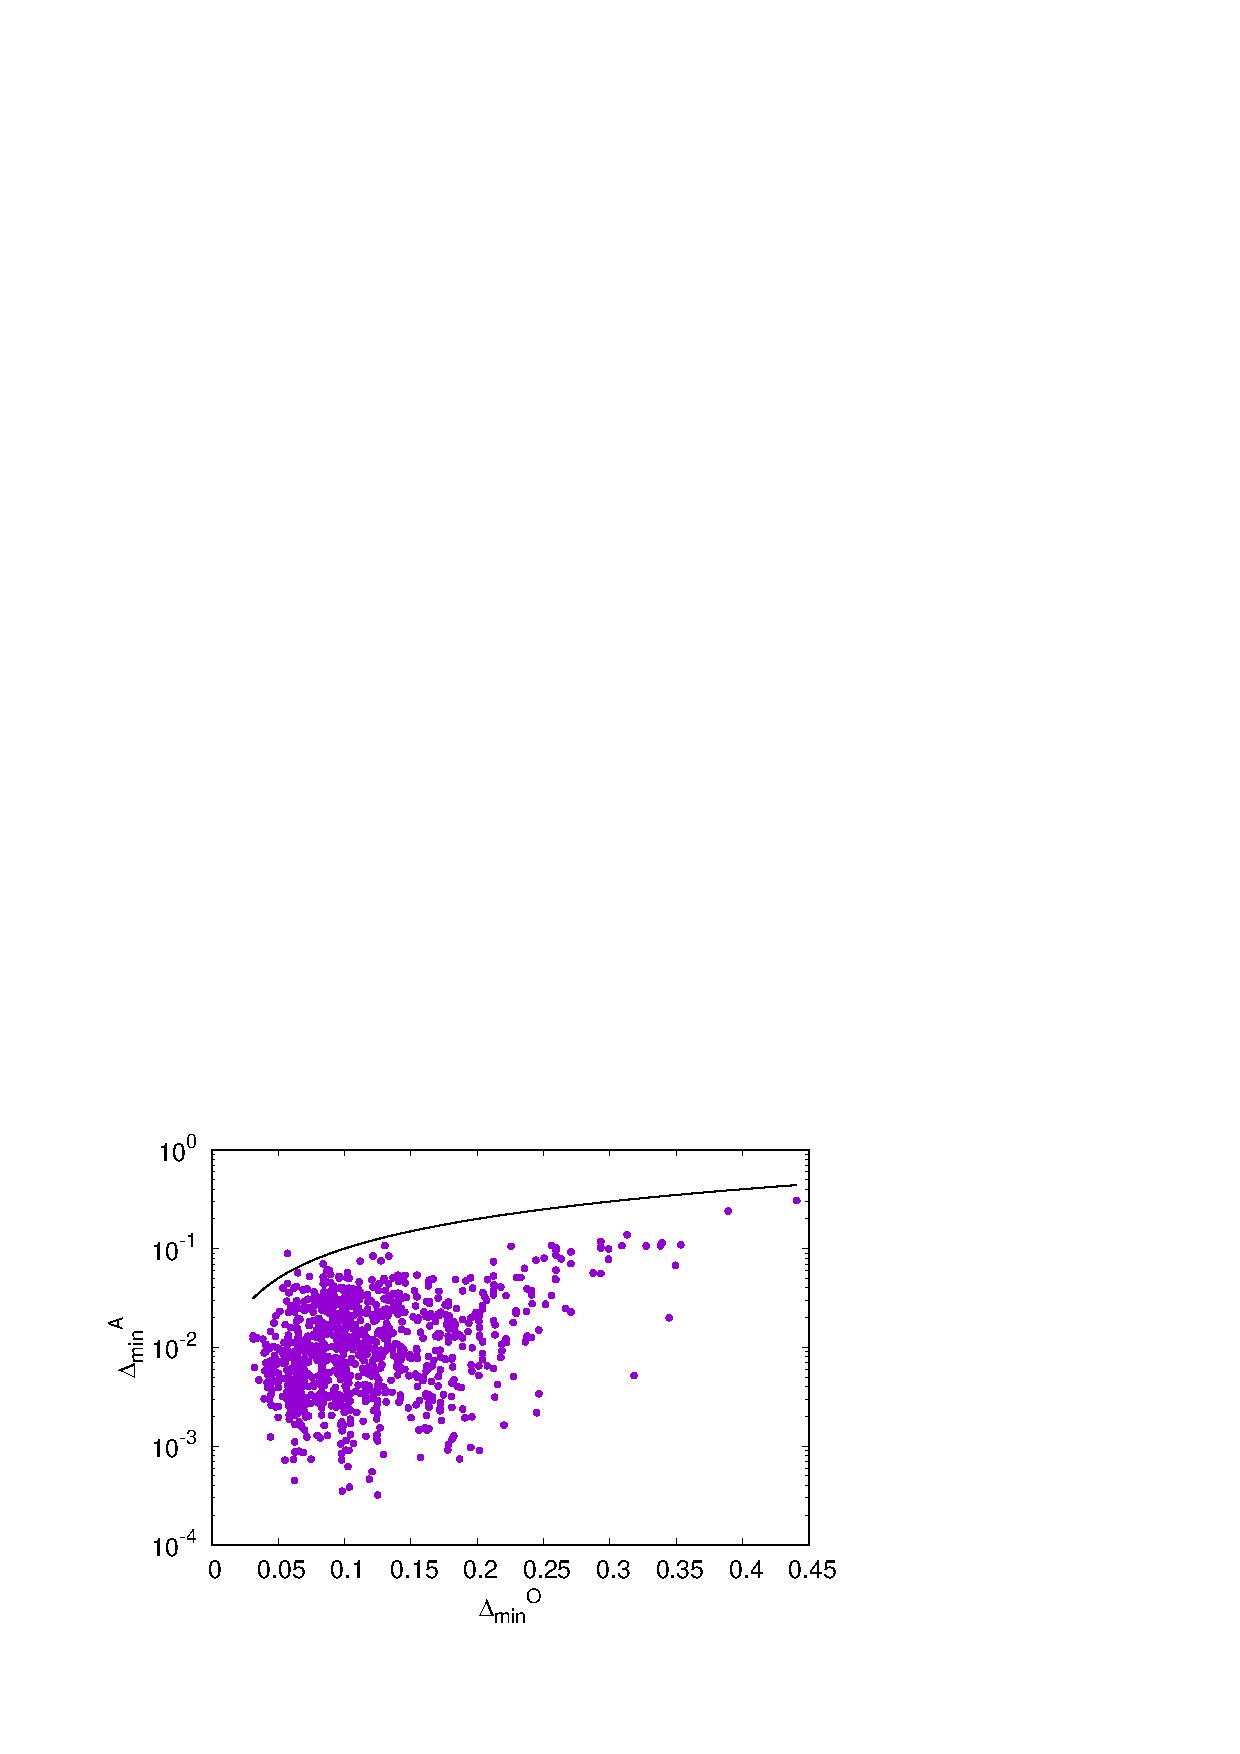
\includegraphics[scale=0.2]{MinGap_A_g0.png}
\caption{A plot of the minimum energy gaps after adding the anti-ferromagnetic trigger with g=0.5 ($\Delta_{min}^A$), with the original minimum energy gaps ($\Delta_{min}^O$). For 99.9\% of the minimum energy gap was found to have decreased after adding the trigger.}
\label{fig:a13}
\end{figure}
As is clear from Fig. (\ref{fig:a13}), for 99.9\% of the cases, the minimum energy gaps reduce after adding the anti-ferromagnetic trigger with strength 0.5. It was also found that 92.3\% of all the cases still had a single anti-crossing between the ground and the first excited state, while for the other 7.7\% of the cases, it increased to 2.

Additionally, for some cases with small energy gaps between the ground state and the first excited state and short annealing times, it was observed that the success probability can also benefit owing to non-adiabatic evolution of the state. As seen in problem 950 in the previous section, for $T_A$=10 the state of the system shifts to the first excited state prior to the minimum gap anti-crossing. The overlap with the ground state can then increase because of the following non-adiabatic processes:
\begin{itemize}
\item If there are no higher energy states close to the state of the system, the wave function of the state can transfer some amplitude back to the ground state, at one of the anti-crossings.
\item If the higher energy states come close to the system state, before it approaches the energy anti-crossing, the system state can further transit to a superposition state of the higher energy levels. This might increase the overlap of the state with the ground state compared to the case where the state closely follows the first excited state after crossing the energy anti-crossing.
\end{itemize}

Thus, when the annealing time is increased to 100 or 1000, the state of the system stays close to the ground state till it reaches the energy anti-crossing, and transitions to the first excited state afterwards. This explains the drop in the percentage of improved cases upon increasing the annealing time after adding the anti-ferromagnetic trigger. \\

To obtain an estimate of the difficulty of the affected problems, Fig. (\ref{fig:a14}) shows a scatter plot of the success probabilities after adding the trigger against the original success probabilities, for the three annealing times. It should be noted that the 43.9\% of the problems improved upon by adding anti-ferromagnetic trigger for $T_A$=10, are the ones that had relatively smaller original success probabilities (harder problems with smaller minimum energy gaps). Adding the anti-ferromagnetic trigger reduces the minimum energy gap, thereby increasing the success probability by either of the two mechanisms listed above.

\begin{figure}[H]
\centering 
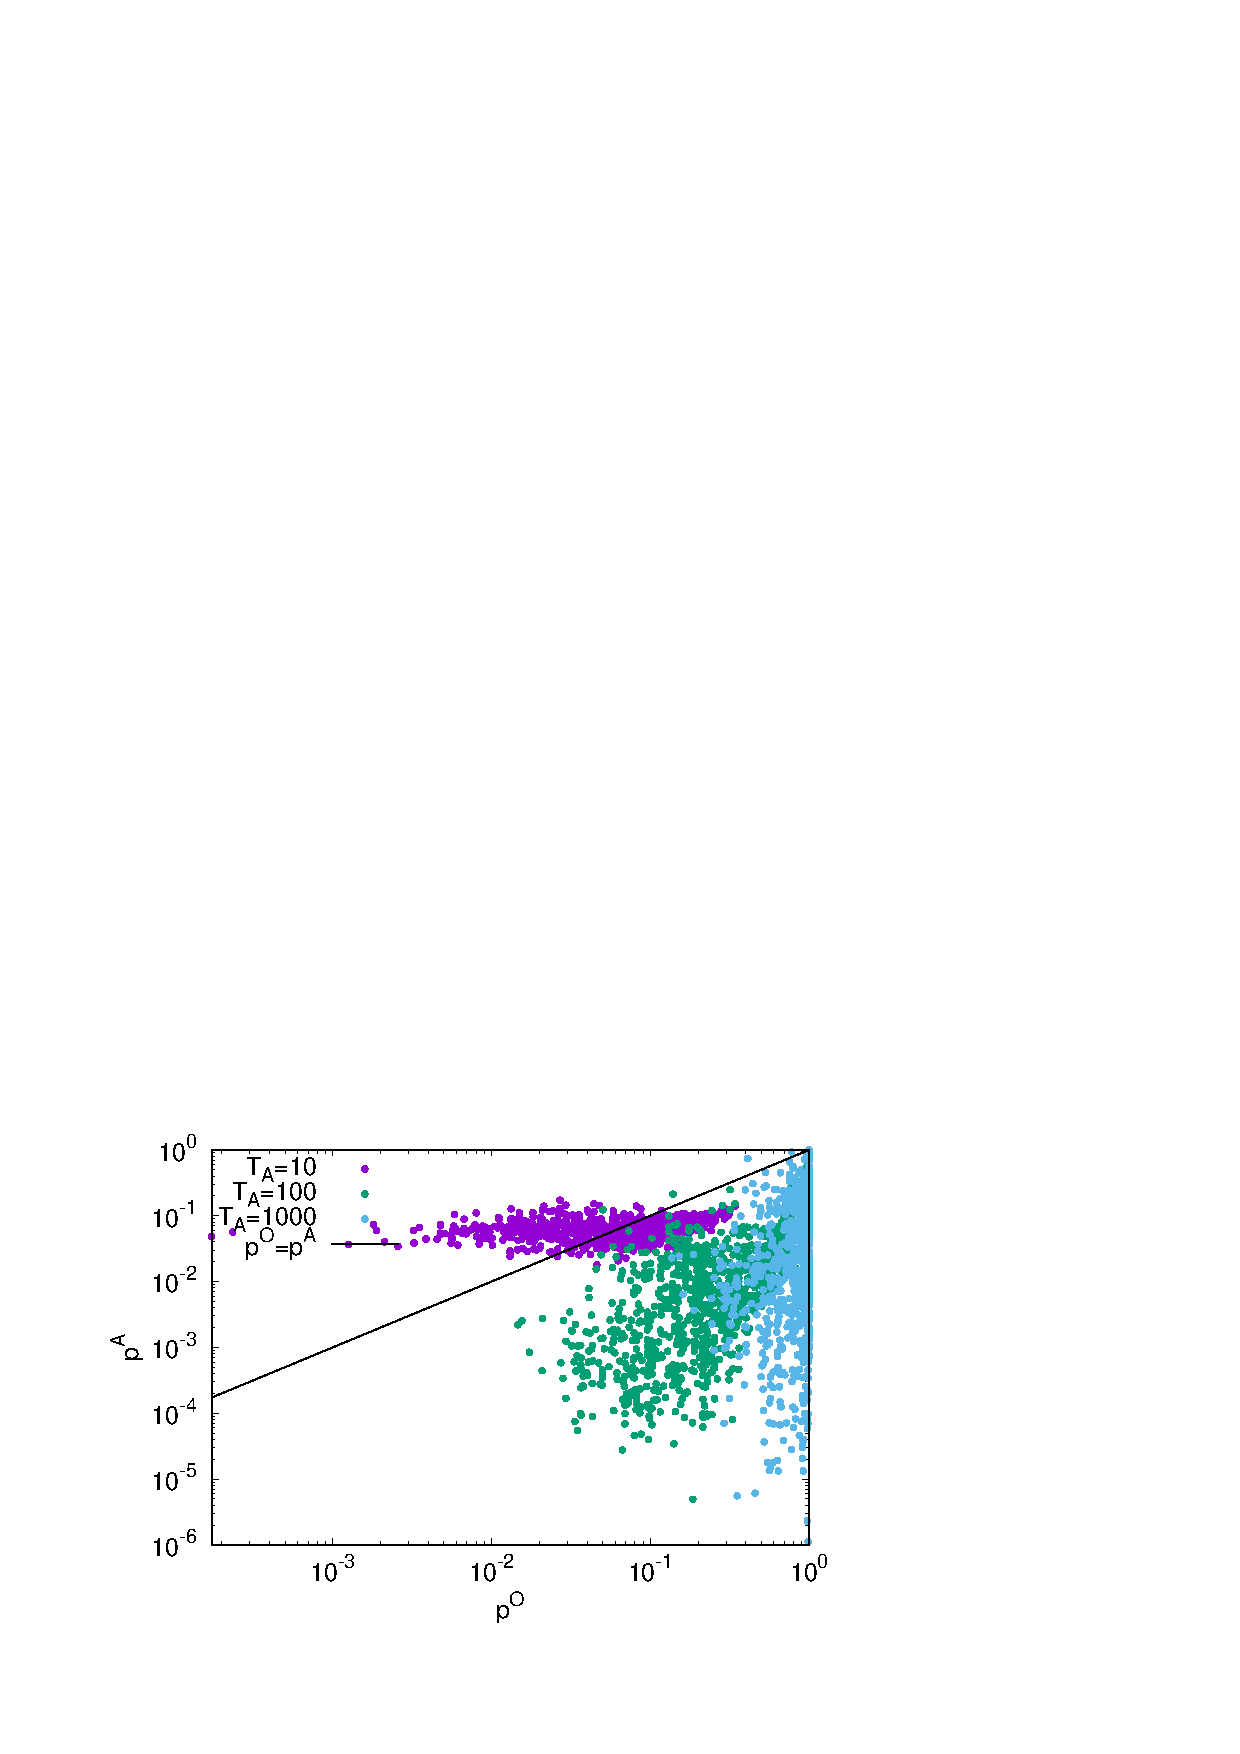
\includegraphics[scale=0.24]{ProbScat_g0.png}
\caption{A plot of the success probabilities after adding the anti-ferromagnetic trigger with g=0.5 ($p^A$), with the original success probabilities($p^O$) for annealing time 10, 100 and 1000.}
\label{fig:a14}
\end{figure}

It should also be noted that for $T_A$=100 and $T_A$=1000, the original success probabilities are already quite high, giving way to another reason for the decrease in the relative success probability with increasing annealing time. \\

For both $T_A$=100 and $T_A$=1000 problems 402 and 709 were found to have a larger relative success ratio upon adding the anti-ferromagnetic trigger with g=0.5. Problem 402 corresponded to the only case where the minimum energy gap had increased after adding the trigger, explaining the reason for the increase in the success probability.\\
For problem 709, Fig. (\ref{fig:a15}) shows the energy gap between the ground energy level and the first excited state of the Hamiltonian (as a function of the annealing parameter), before and after adding the anti-ferromagnetic trigger. The inset of the figure also shows the energy gaps for some other problems after adding the trigger. As can be observed in the figure, the shape of the curve after adding the anti-ferromagnetic trigger to problem 709 is different from both the original Hamiltonian and the other problems. The slope in this case, unlike the other cases, is not symmetric about the minimum gap value. While comparing the success probabilities across different problems (and assuming $p=1-e^{-\dfrac{-T {\Delta}^2}{c}}$), the slope (c) for  each problem was supposed to have a similar structure and only changes in the minimum gaps were accounted for. Since this assumption breaks down for this case, and the Landau-Zener formula is no longer does not hold good for this problem.\\

\begin{figure}[H]
\centering 
\includegraphics[scale=0.24]{Mingap_709_g0_A.png}
\caption{A comparison of the minimum energy gaps between the two lowest energy levels as a function of the annealing parameter, in the absence and presence of the anti-ferromagnetic trigger with g=0.5. The inset shows a comparison with some other problems after adding the trigger. The key difference in case of problem 709 is that the slope of the curve is not symmetric about the point of minimum gap, unlike all other cases. }
\label{fig:a15}
\end{figure}

Finally, for checking if the dynamics during the evolution of the state under the action of the anti-ferromagnetic trigger is adiabatic, equation (\ref{eq:lz3}) should be verified, as was done in the last chapter. We plotted the success probability against the minimum energy gaps for all the problems of the set, before and after adding the ferromagnetic trigger, for all the three annealing times. The resulting plot is shown in Fig. (\ref{fig:a17}).

\begin{figure}[H]
\centering 
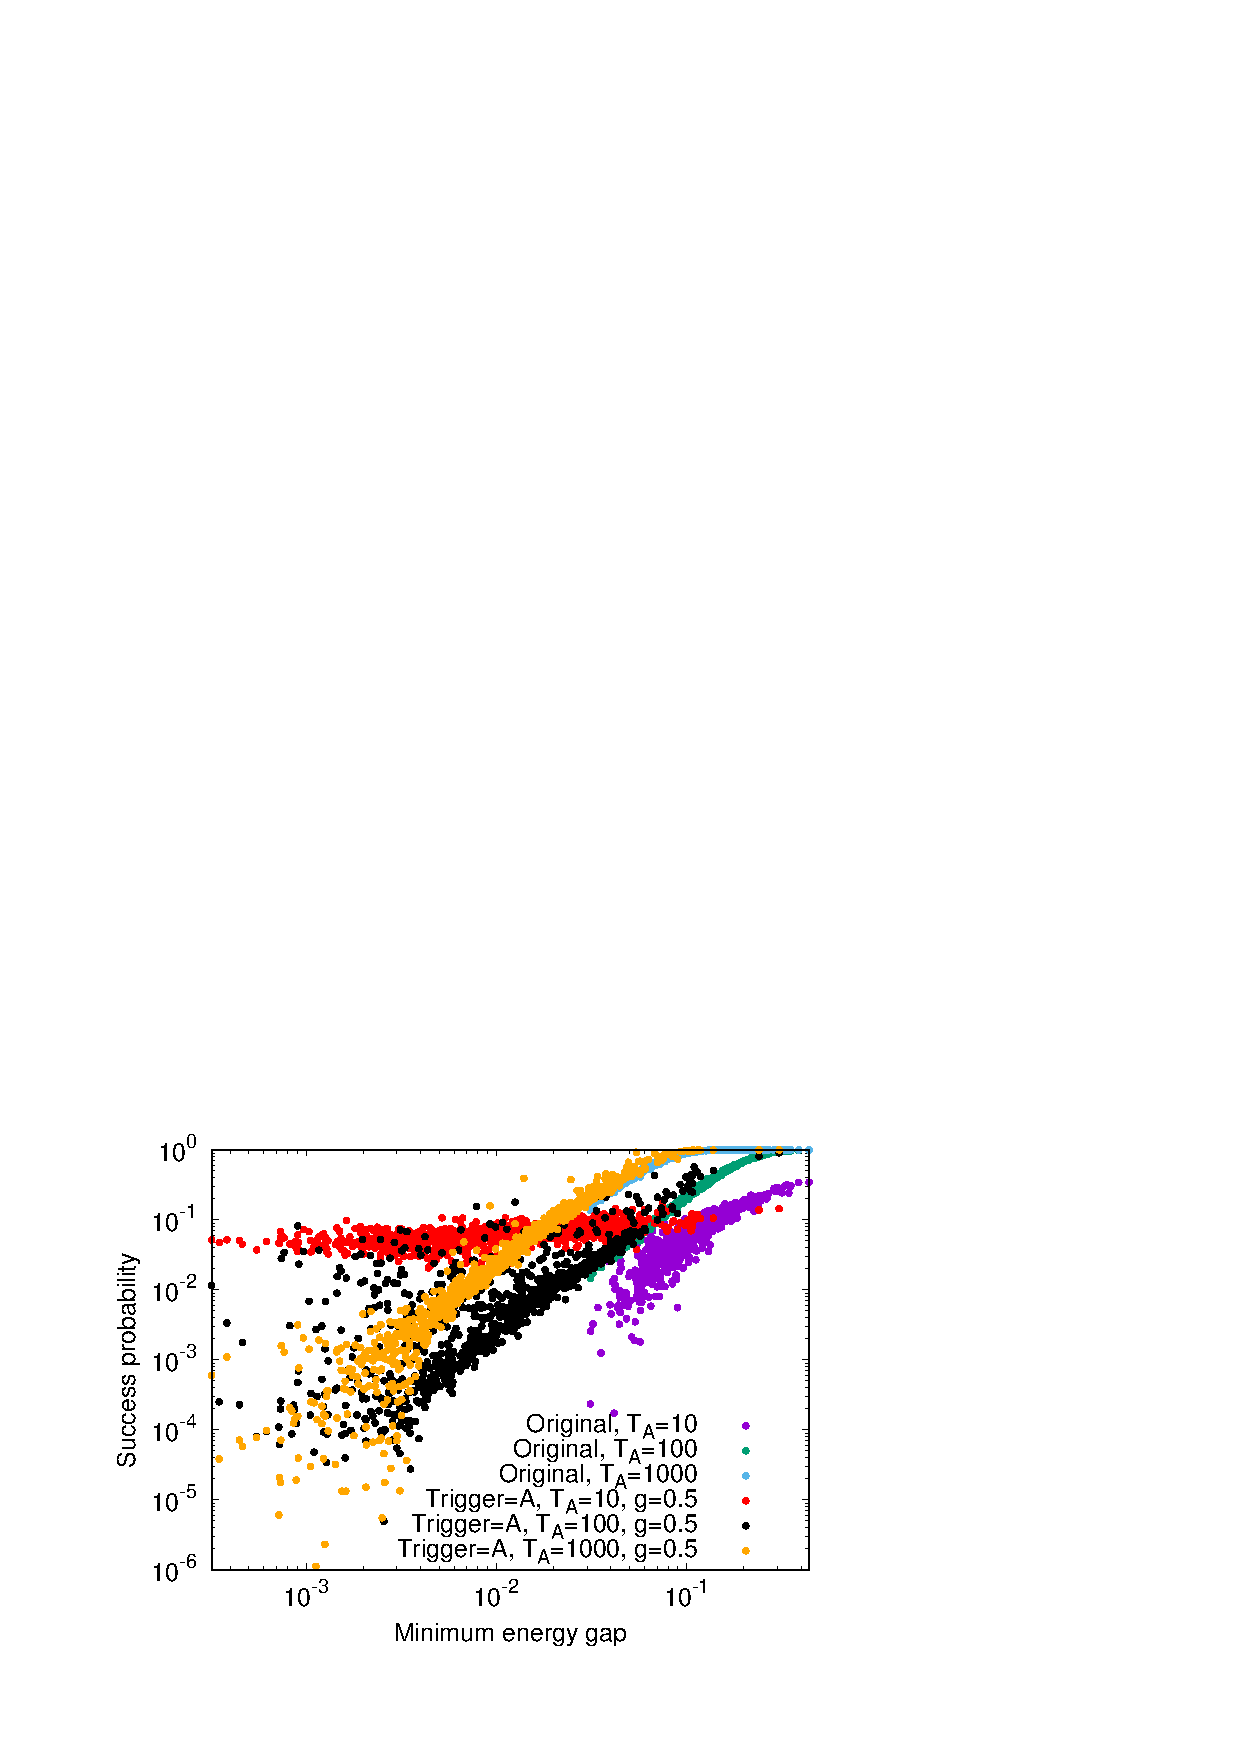
\includegraphics[scale=0.24]{SuccVsGap_OA_g0.png}
\caption{Success probability versus minimum energy plot for all the problems belonging to the set of 12-spin SAT problems, for annealing times 10, 100 an 1000, in the absence and presence of ferromagnetic trigger.}
\label{fig:a17}
\end{figure}


It can be noted from Fig. (\ref{fig:a17}) that the original success probabilities mostly follow the Landau-Zener dependence on minimum energy gaps, although the scattering for $T_A$=10 is comparatively large. As the annealing time is increased, the scattering becomes less prominent. However, upon adding the trigger, the scattering becomes even larger, so that the points corresponding to $T_A$=10 appear rather flat. Also, for smaller gaps, these points have a higher success probability than the points corresponding to $T_A$=100, due to non-adiabatic evolution. Although in this case too the curves become successively less scattered by increasing the annealing time, the general effect of adding the trigger with strength g=0.5 is to shift the points leftwards by reducing the minimum energy gaps.


\section*{g=1}
In this section, will feature the same analysis as the last section but with the value of the strength parameter set to 1. We begin by showing the distribution of the relative success probability after adding the anti-ferromagnetic trigger with g=1, for annealing times 10, 100 and 1000, in Figs. (\ref{fig:a18}), (\ref{fig:a19}) and (\ref{fig:a20}) respectively.

\begin{figure}[H]
\centering 
\includegraphics[scale=0.24]{A_T10_g1.png}
\caption{Distribution of the relative success probability $\dfrac{p^A}{p^O}$ for $T_A$=10. 37.7\% of the cases were found to have a higher success probability after adding the trigger.}
\label{fig:a18}
\end{figure}
\begin{figure}[H]
\centering 
\includegraphics[scale=0.24]{A_T100_g1.png}
\caption{Distribution of the relative success probability $\dfrac{p^A}{p^O}$ for $T_A$=100. 21.5\% of the cases were found to have a higher success probability after adding the trigger. }
\label{fig:a19}
\end{figure}
\begin{figure}[H]
\centering 
\includegraphics[scale=0.24]{A_T1000_g1.png}
\caption{Distribution of the relative success probability $\dfrac{p^A}{p^O}$ for $T_A$=1000. 20\% of the cases were found to have a higher success probability after adding the trigger.}
\label{fig:a20}
\end{figure}

37.7\% of the cases had an improved success probability after adding the anti-ferromagnetic trigger for $T_A$=10. This percentage reduced to 21.5\% and 20\% upon increasing the annealing time to 100 and 1000 respectively. Moreover, as the annealing time was increased, the largest value of the relative success probability dropped from 501 at $T_A$=10, to 15.85 at $T_A$=100, to 6.31 at $T_A$=1000. Again, for obtaining more insights about the effects of adding the anti-ferromagnetic trigger with g=1, the minimum energy gaps were computed for all the problems of the set after adding the trigger. Fig. (\ref{fig:a21}) shows the resulting scatter plot between the minimum energy gap after adding the anti-ferromagnetic trigge against the original minimum energy gaps.

\begin{figure}[H]
\centering 
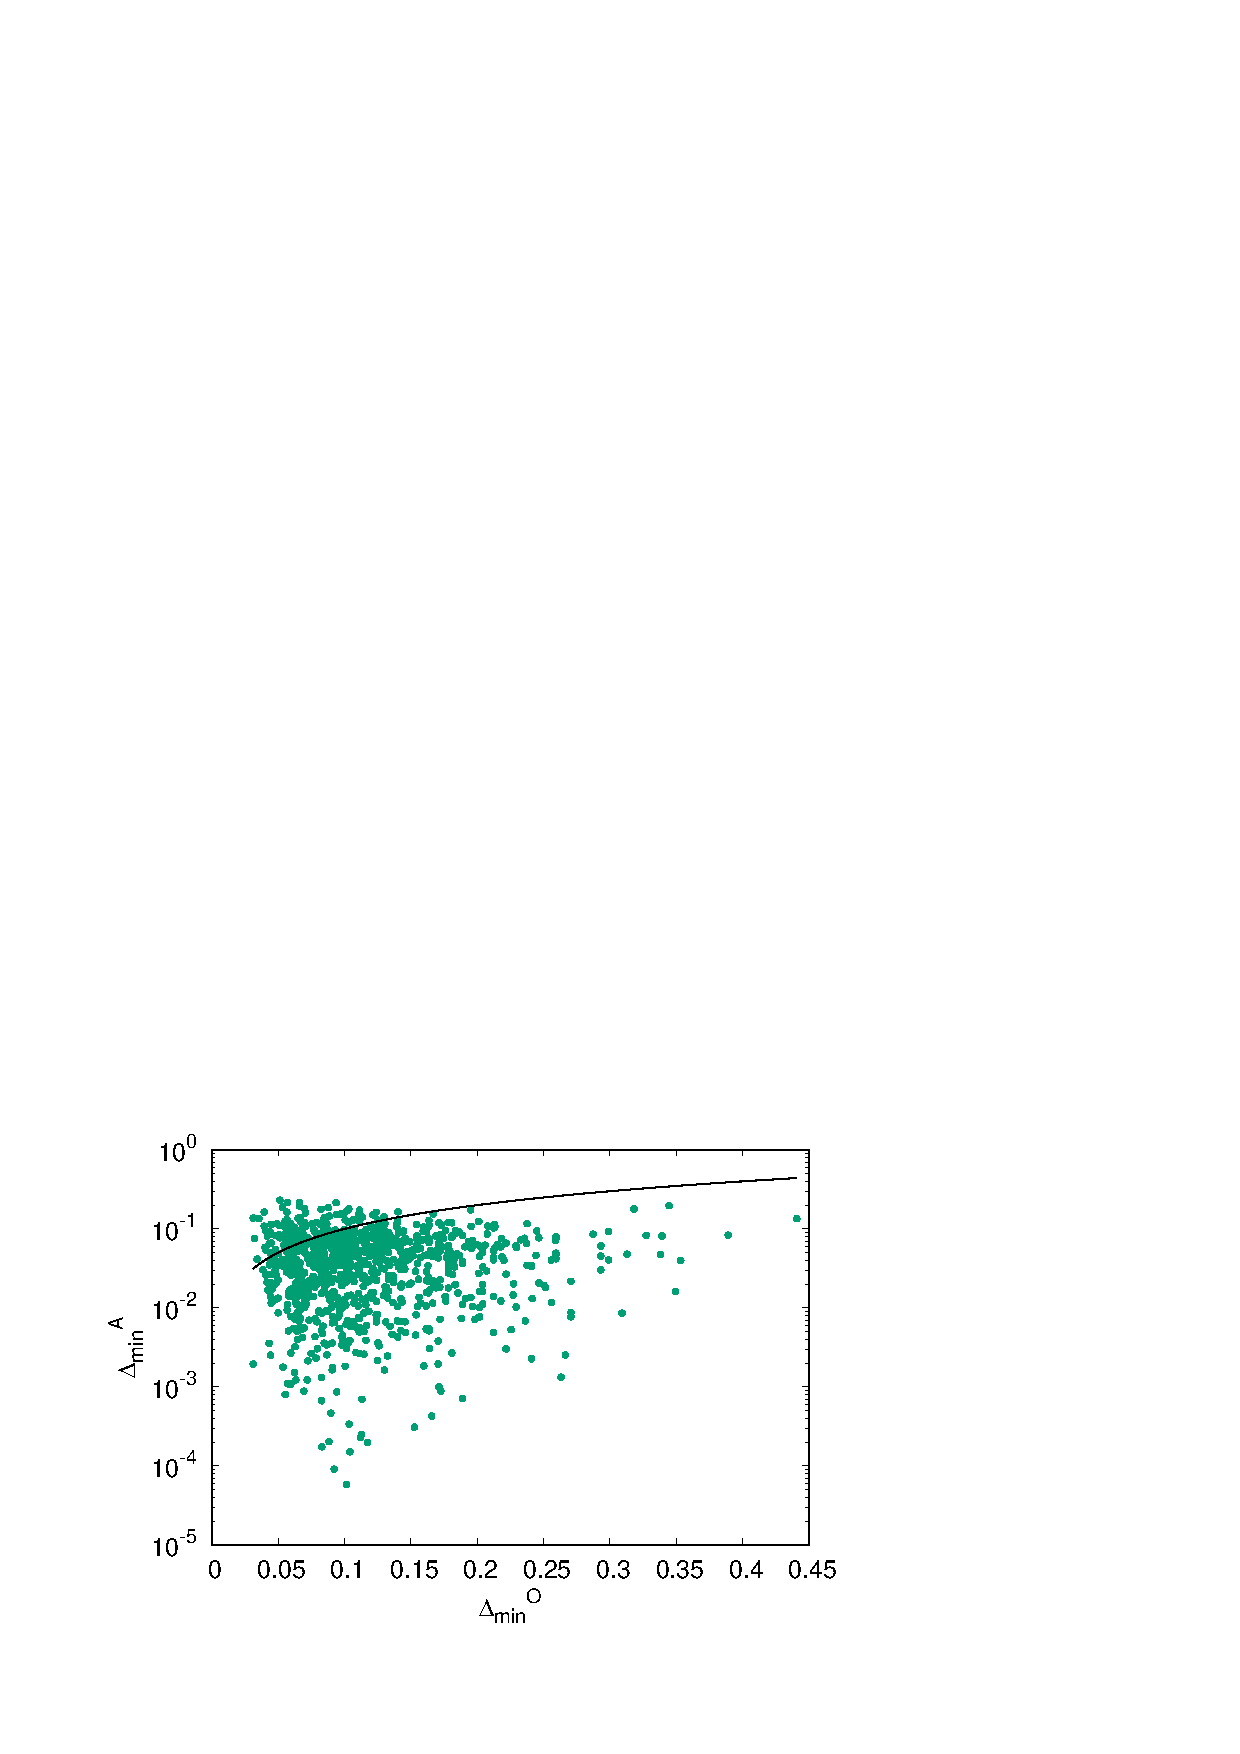
\includegraphics[scale=0.2]{MinGap_A_g1.png}
\caption{A plot of the minimum energy gaps after adding the anti-ferromagnetic trigger with g=1 ($\Delta_{min}^A$), with the original minimum energy gaps ($\Delta_{min}^O$). For 87.9\% of the minimum energy gap was found to have decreased after adding the trigger.}
\label{fig:a21}
\end{figure}
In this case 87.9\% of the cases were found to have smaller minimum energy gaps upon the addition of the trigger. Thus, a decrease in the success probability for most of the cases compared to the original seems to be plausible.

Furthermore, for most of the cases the number of  energy anti-crossings between the ground state and the first excited state increased to 2, while in one case it was noted to be 4. Tab. (\ref{tab:a4}) shows the number of cases with different number of anti-crossings.

\begin{table}[H]
\centering
\renewcommand{\arraystretch}{1.5}
\begin{tabular}{|c|c|}
\hline 
Number of anti-crossings & Number of cases (\%) \\ 
\hline 
1 & 20.2 \\ 
\hline 
2 & 70.5 \\ 
\hline 
3 & 9.2 \\ 
\hline 
4 & 0.1 \\ 
\hline 
\end{tabular} 
\caption{Number of cases with different number of anti-crossings after adding the anti-ferromagnetic trigger.}
\label{tab:a4}

\end{table}
For obtaining an estimate for the difficulty of the problems which have a relative success ratio greater than one, a scatter plot of the original success probability and that after adding the anti-ferromagnetic trigger has been shown in Fig. (\ref{fig:a22}).


\begin{figure}[H]
\centering 
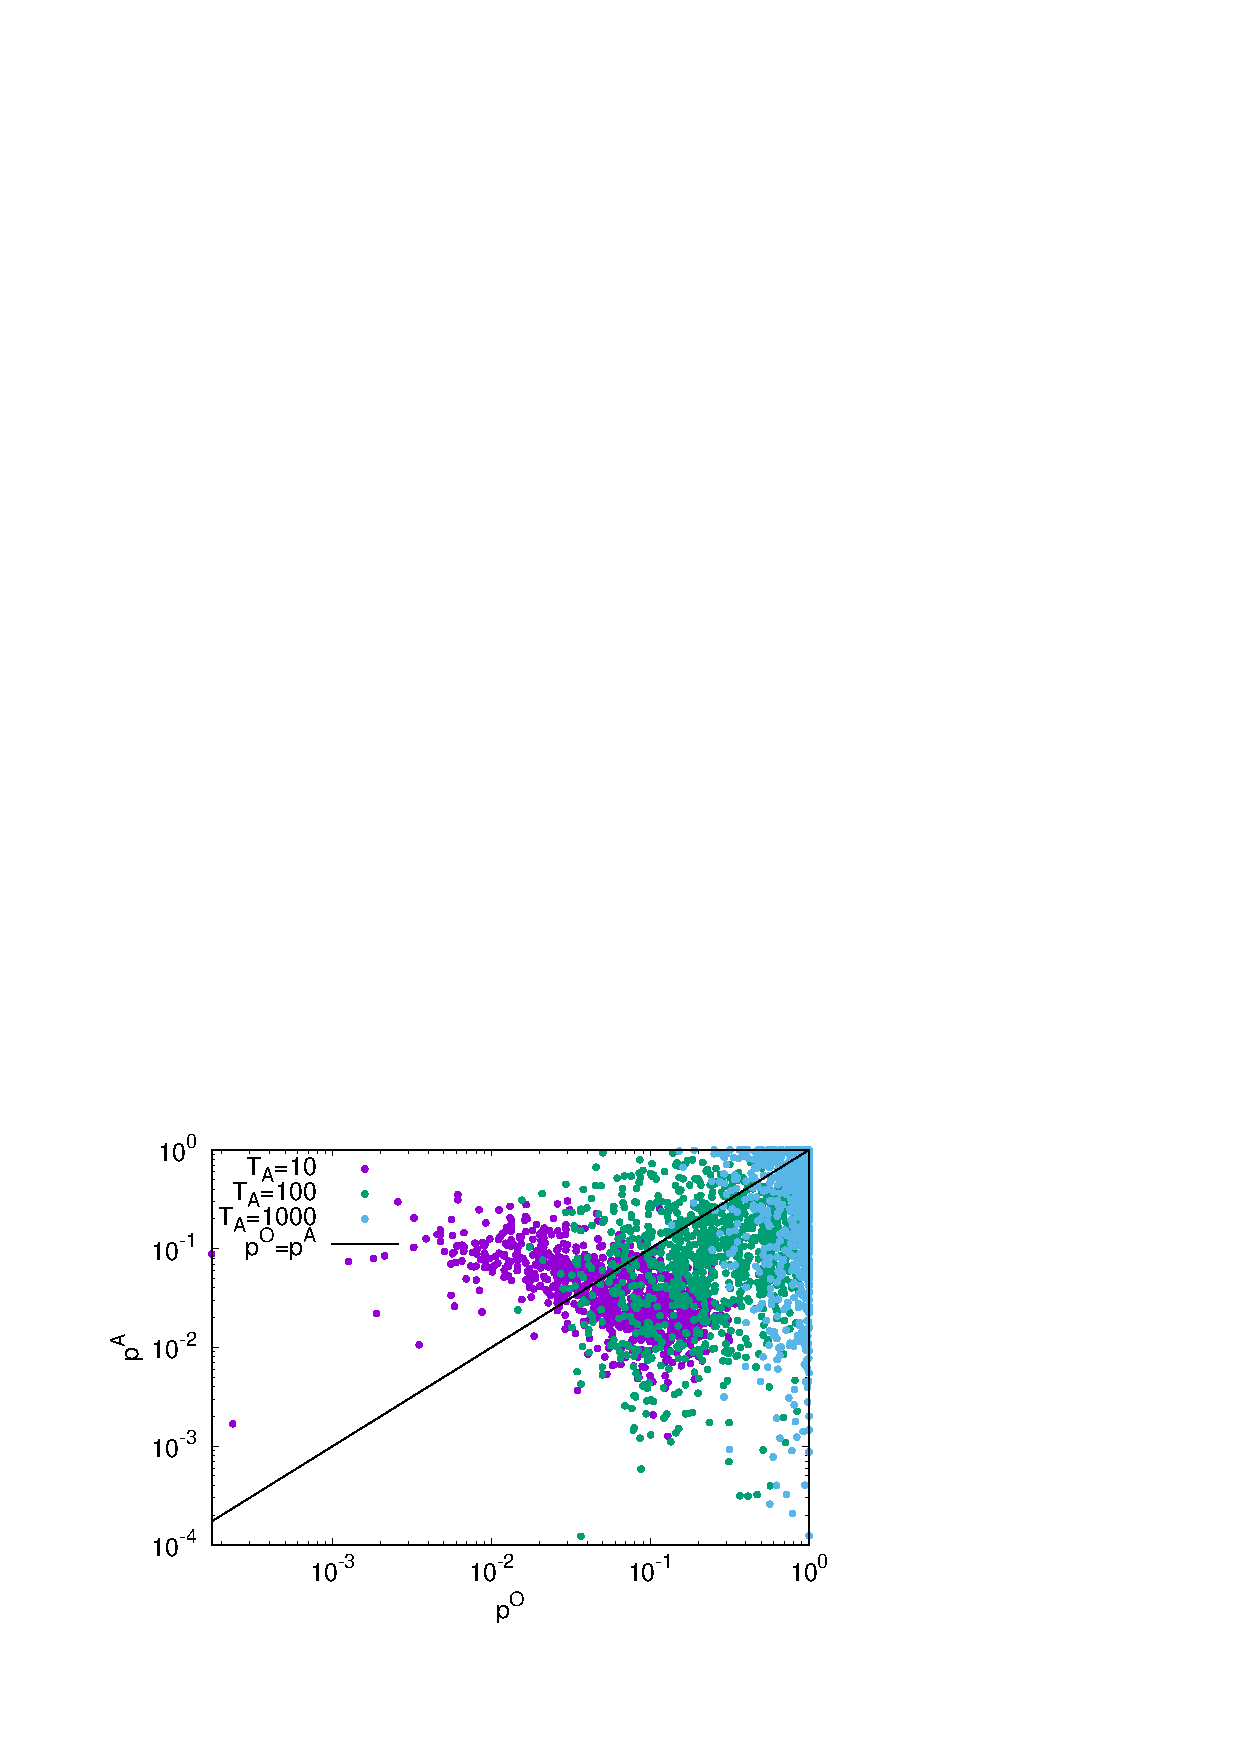
\includegraphics[scale=0.24]{ProbScat_g1.png}
\caption{A plot of the success probabilities after adding the anti-ferromagnetic trigger with g=1 ($p^A$), with the original success probabilities ($p^O$) for annealing time 10, 100 and 1000.}
\label{fig:a22}
\end{figure}

Again, it can be noted that for $T_A$=10, the 37.7\% of the problems that have a higher success probability after adding the anti-ferromagnetic trigger are limited to the cases with smaller original success probability (smaller gaps). Since adding the trigger reduces the minimum energy gap in most of the cases, the cases with smaller $p^O$ benefit from a non-adiabatic evolution (shorter annealing time).\\

For understanding the role that the annealing time plays in improving the success probability, the scatter plots for the minimum energy gaps was plotted again, but only for the problems with a relative success probability greater than 1 for a fixed annealing time. Figs. (\ref{fig:a23}), (\ref{fig:a26}) and (\ref{fig:a27}) show the resulting plots for an annealing time of 10, 100 and 1000 respectively.\\

In the 37.7\% of the cases with higher success probability after adding the trigger for $T_A$=10, 27.9\% of the cases were found to have smaller minimum gaps as a result of adding the trigger. These cases can therefore be expected to be the ones benefiting from the non-adiabatic evolution for small annealing time of $T_A$=10. On the other hand, for the rest 9.8\% of the cases the minimum gaps were increased. It was noted that except for 2 cases (problems 325 and 705), all the problems with enlarged minimum gap and improved success probability for $T_A$=10 also had improved success probability for $T_A$=100 and $T_A$=1000. This suggests that for these cases adding the anti-ferromagnetic trigger increased the minimum energy gap enough to make the evolution closer to adiabatic even for $T_A$=10. 

Additionally, for problems 325 and 705, the relative success probability was greater than 1 for $T_A$=10 and $T_A$=1000, while it was smaller than 1 for $T_A$=100. It was found that the energy spectra and the mechanism leading to this trend were similar for both these problems. Therefore, Figs. (\ref{fig:a24}) and (\ref{fig:a25}) show the energy spectrum and the energy expectation values for the state, before and after adding the trigger for problem 705.

\begin{figure}[H]
\centering 
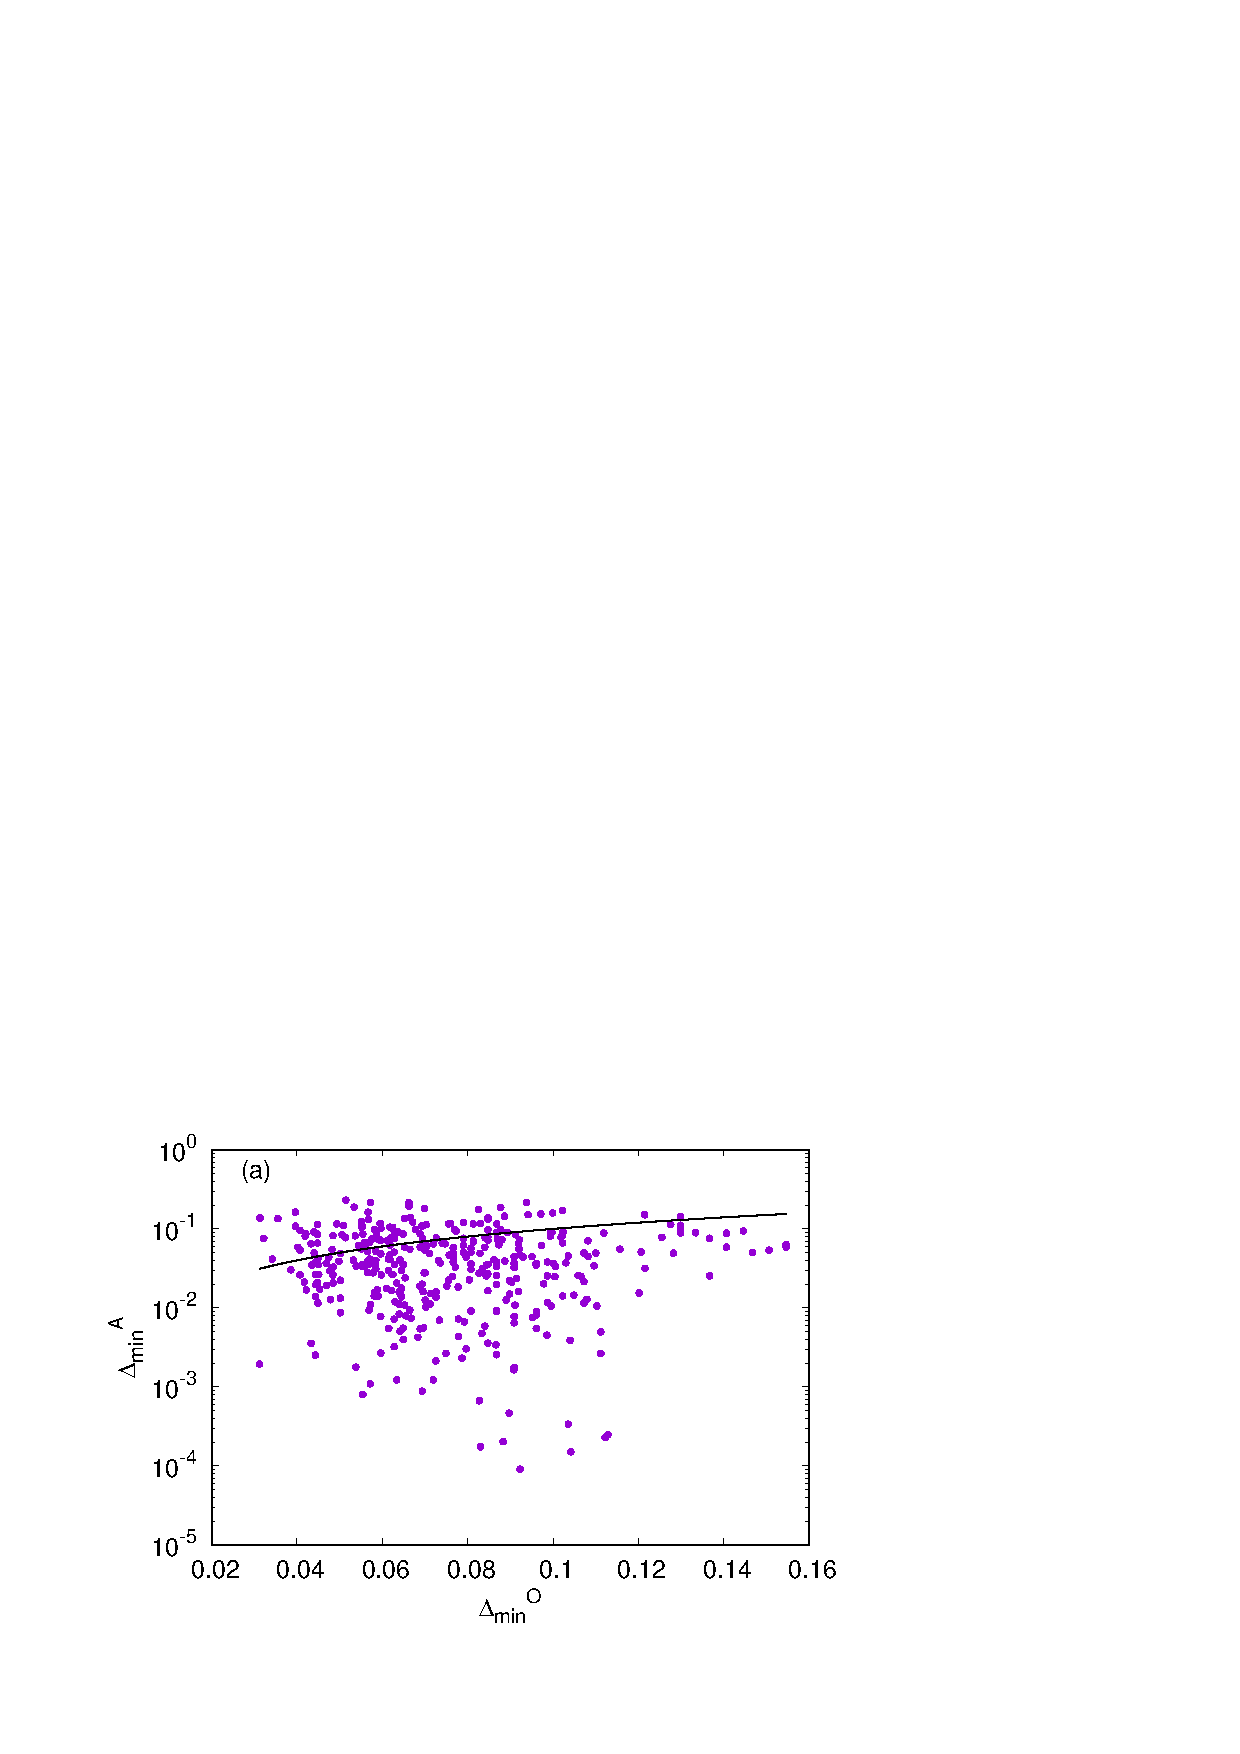
\includegraphics[scale=0.22]{selected_T10_g1.png}
\caption{For the cases with higher success probability for $T_A$=10 after adding the anti-ferromagnetic trigger with g=1, the scatter plot of energy gaps $\Delta^A $ with $\Delta^O$. 279 out of 377 of such cases were found to have smaller minimum energy gaps after adding the trigger.}
\label{fig:a23}
\end{figure}

\begin{figure}[H]
\centering 
\includegraphics[scale=0.24]{705_O_T.png}
\caption{Energy spectrum and energy expectation values for the instantaneous state for the original Hamiltonian in problem 705. }
\label{fig:a24}
\end{figure}
\begin{figure}[H]
\centering 
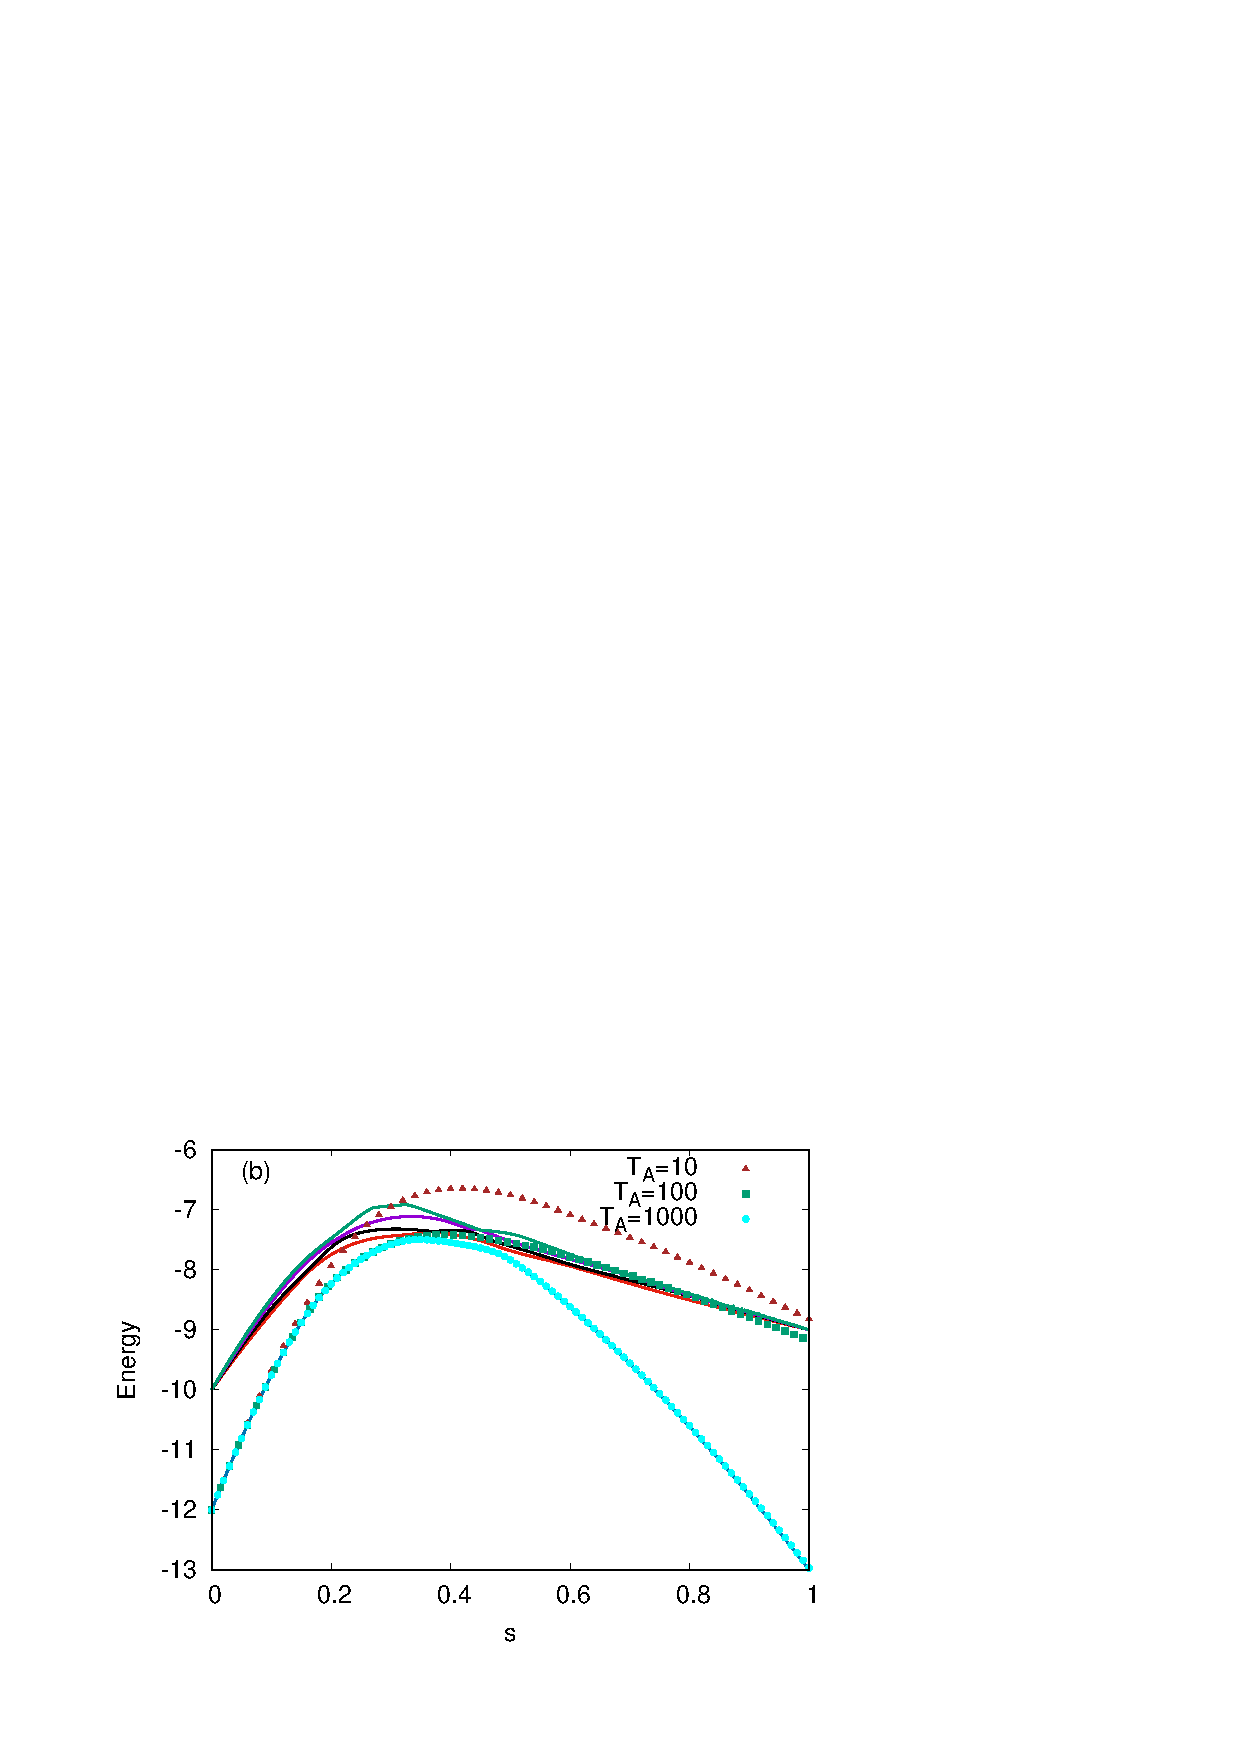
\includegraphics[scale=0.24]{705_A_T_g1.png}
\caption{Energy spectrum and energy expectation values for the instantaneous state for the Hamiltonian after adding the anti-ferromagnetic trigger to problem 705.}
\label{fig:a25}
\end{figure}
Although adding the trigger enlarges the minimum gap in these cases, the spectrum of the problem is changed in a way that the higher energy levels remain closer to the ground state. This gives the state a chance to transition to the higher energy levels even before the first energy anti-crossing for $T_A$=10, and coincidentally end in a state with larger overlap with the ground state than in the original case where it closely follows the first excited state after the anti-crossing. For $T_A$=100, and in the presence of the trigger, the state shifts to the higher excited state at the second energy anti-crossing, but this time the overlap of the final state with the ground state is smaller than that in the case of the original Hamiltonian. Finally, an annealing time of $T_A$=1000 becomes long enough for the evolution to become adiabatic, and since the minimum energy gap is increased after adding the trigger, the success probability in the presence of the trigger becomes larger.\\

Next, from Figs. (\ref{fig:a26}) and (\ref{fig:a27}) it can be noted that the majority of the problems improved by adding anti-ferromagnetic trigger, and choosing the annealing time to be $T_A$=100 or $T_A$=1000 correspond to the cases where the minimum energy gaps became larger upon adding the trigger. 117 of the   215 cases improved after adding the trigger for $T_A$=100, and 121 of the 200 cases for $T_A$=1000 had larger minimum gaps after including the trigger.
\begin{figure}[H]
\centering 
\includegraphics[scale=0.35]{selected_T100_g1.png}
\caption{For the cases with higher success probability for $T_A$=100 after adding the anti-ferromagnetic trigger with g=1, the scatter plot of energy gaps $\Delta^A $ with $\Delta^O$. 117 out of 215 of such cases were found to have larger minimum energy gaps after adding the trigger. Some of the other 98 cases studied have been marked.}
\label{fig:a26}
\end{figure}
\begin{figure}[H]
\centering 
\includegraphics[scale=0.35]{selected_T1000_g1.png}
\caption{For the cases with higher success probability for $T_A$=1000 after adding the anti-ferromagnetic trigger with g=1, the scatter plot of energy gaps $\Delta^A $ with $\Delta^O$. 121 out of 200 of such cases were found to have larger minimum energy gaps after adding the trigger. Some of the other 79 cases studied have been marked.}
\label{fig:a27}
\end{figure}
Some of the problems with improved success probability despite of reduced minimum energy gaps were selected and their dynamics was studied. These have been marked in Figs. (\ref{fig:a26}) and (\ref{fig:a27}). It can noticed that problems 275, 441, 709, 950 and 983 occur appear in both the figures. Following are the conclusions after studying these cases individually.
\begin{itemize}
\item For problems 70, 275, 441, 709 and 864, the presence of two anti-crossings increases the overlap of the final state with the ground state of the Hamiltonian.  Figs. (\ref{fig:a28}) and (\ref{fig:a29}) respectively show the energy spectrum and the energy expectation values for the corresponding state for the original Hamiltonian, and the Hamiltonian after adding the anti-ferromagnetic trigger.


\begin{figure}[H]
\centering 
\includegraphics[scale=0.24]{441_O_T100_1000.png}
\caption{Energy spectrum and energy expectation values for the state for original Hamiltonian in problem 441.}
\label{fig:a28}
\end{figure}
\begin{figure}[H]
\centering 
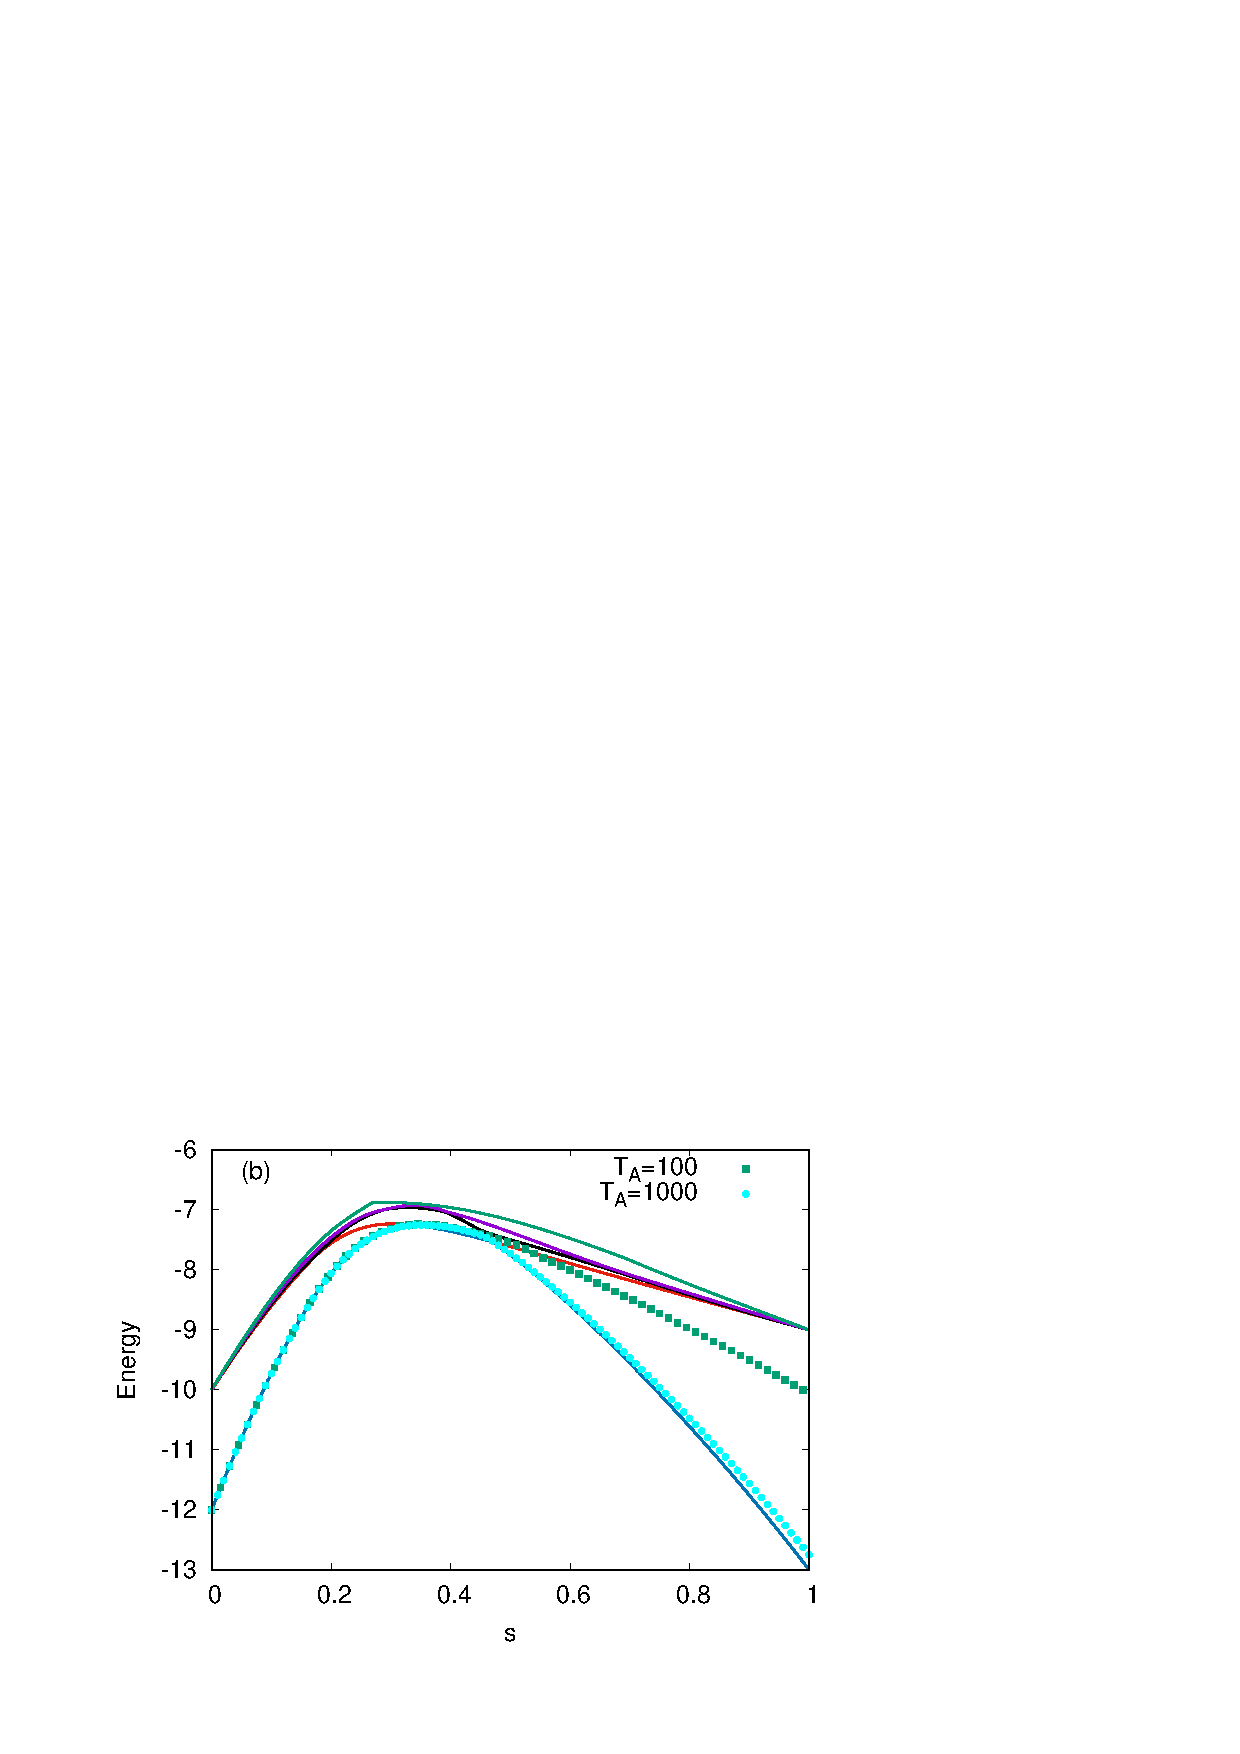
\includegraphics[scale=0.24]{441_A_g1_T100_1000.png}
\caption{Energy spectrum and energy expectation values for the state of the Hamiltonian after adding the anti-ferromagnetic trigger to problem 441 with g=1.}
\label{fig:a29}
\end{figure}

After adding the trigger to this problem, and for both $T_A$=100 and $T_A$=1000, the system state shifts most of its amplitude to the first excited state at the first anti-crossing. On reaching the second anti-crossing, some of the amplitude of the state comes back to the ground state, thus increasing the success probability in these cases.

\item For understanding the reasons for improved success probability in problem 950, the instantaneous overlap of the state of the system was computed with the ground, first excited and second excited state of the Hamiltonian, for $T_A$=100. 

\begin{figure}[H]
\centering
  \includegraphics[scale=0.24]{950_s12_O.png}
  \label{fig:a30}
  \caption{The energy spectrum and energy expectation values for the state of the Hamiltonian in problem 950.}
 \end{figure}

\begin{figure}[H]
  \centering
  \includegraphics[scale=0.24]{950_Overlap_Orig.png}
  \label{fig:a31}

\caption{Overlap of the instantaneous state with the ground state and the first excited state of the Hamiltonian in problem 950, for $T_A$=100.}
\end{figure}
As can be observed on comparing Fig. (\ref{fig:a30}) with Fig. (\ref{fig:a32}) the energy spectrum of problem 950 changes significantly upon adding the anti-ferromagnetic trigger. The minimum energy gap becomes smaller, and the two lowest energy states remain in close vicinity for longer. Unlike the shift of the state of the system to the first excited state at the anti-crossing, and following it closely thereafter in the original Hamiltonian for $T_A$=100 (see Fig. (\ref{fig:a31})), the dynamics of the state is more complex in case of including the anti-ferromagnetic trigger. It can be noted from Fig. (\ref{fig:a33}) that upon adding the trigger the system transits to the first excited state at the anti-crossing, from where it shifts most of its amplitude to the second excited state. The remaining amplitude in the first excited state transitions back to the ground state, improving the success probability. Similar dynamics can be expected to benefit the case for $T_A$=1000 case as well.
\begin{figure}[H]
\centering
  \includegraphics[scale=0.24]{950_s12_A_g1.png}
  \label{fig:a32}
  \caption{The energy spectrum and energy expectation values for the state after adding the anti-ferromagnetic trigger to Hamiltonian in problem 950.}
 \end{figure}

\begin{figure}[H]
  \centering
  \includegraphics[scale=0.24]{950_A_g1_Overlap.png}
  \label{fig:a33}

\caption{Overlap of the instantaneous state with the ground state and the first excited state of the Hamiltonian after adding anti-ferromagnetic trigger to problem 950.}
\end{figure}

\item Again, for understanding the exact dynamics in case of problem 969, the instantaneous overlap with the three lowest energy levels of the Hamiltonian was computed. As was the case in the original Hamiltonian of problem 950, from Fig. (\ref{fig:a47}) and (\ref{fig:a48}) it can be observed that the system state shifts most of its amplitude to the first excited state at the anti-crossing, after which it stays close to the first excited state for the rest of the course. This decreases the its overlap with the ground state, thus explaining the small success probability.
\begin{figure}[H]
\centering
  \includegraphics[scale=0.24]{969_O_T100.png}
  \label{fig:a47}
  \caption{The energy spectrum and energy expectation values for the state of the Hamiltonian in problem 969.}
 \end{figure}

\begin{figure}[H]
  \centering
  \includegraphics[scale=0.24]{969_Overlap_Orig.png}
  \label{fig:a48}

\caption{Overlap of the instantaneous state with the ground state and the first excited state of the Hamiltonian in problem 969, for $T_A$=100.}
\end{figure}
Fig. (\ref{fig:a50}) makes it clear that the system state shifts to the first excited state at the first anti-crossing. It shifts the amplitude further to the close lying higher excited states. However, since the first and second excited states stay close enough for a long time, so that the state exchanges the amplitude between these states, the overlap with these states oscillates. As the state approaches the second anti-crossing, the amplitude present in the second excited state shifts back to ground state.
\begin{figure}[H]
\centering
  \includegraphics[scale=0.24]{969_A_T100_g1.png}
  \label{fig:a49}
  \caption{The energy spectrum and energy expectation values for the state after adding the anti-ferromagnetic trigger to Hamiltonian in problem 969.}
 \end{figure}

\begin{figure}[H]
  \centering
  \includegraphics[scale=0.24]{969_A_g1_Overlap.png}
  \label{fig:a50}

\caption{Overlap of the instantaneous state with the ground state and the first excited state of the Hamiltonian after adding anti-ferromagnetic trigger to problem 969.}
\end{figure}
\item  Finally, for problem 983, Fig. (\ref{fig:a51}) shows theenergy gap between the lowest two energy levels as a function of the annealing parameter, for the original Hamiltonian, and that after adding the anti-ferromagnetic trigger. It can be noted that the compared to minimum energy gap in the original Hamiltonian, the energy gap after adding the trigger becomes more wider, so that the ground state and the first excited state stay close for longer. This gives the state to oscillate the amplitude between these states. Therefore, despite the decrease in the minimum energy gap, there is more amplitude in the ground state in this case, compared to that in the original Hamiltonian.

\begin{figure}[H]
  \centering
  \includegraphics[scale=0.24]{983_Mingap.png}
  \label{fig:a51}

\caption{Energy gap between the ground state and the first excited state of the original Hamiltonian, and that after adding the anti-ferromagnetic trigger with g=1.}
\end{figure}
\end{itemize}


Again, for checking if the dynamics after adding the anti-ferromagnetic trigger with g=1 was adiabatic, the success probabilities for different problems were plotted against the corresponding minimum gaps. Fig. (\ref{fig:a34}) shows the resulting plot.

\begin{figure}[H]
\centering 
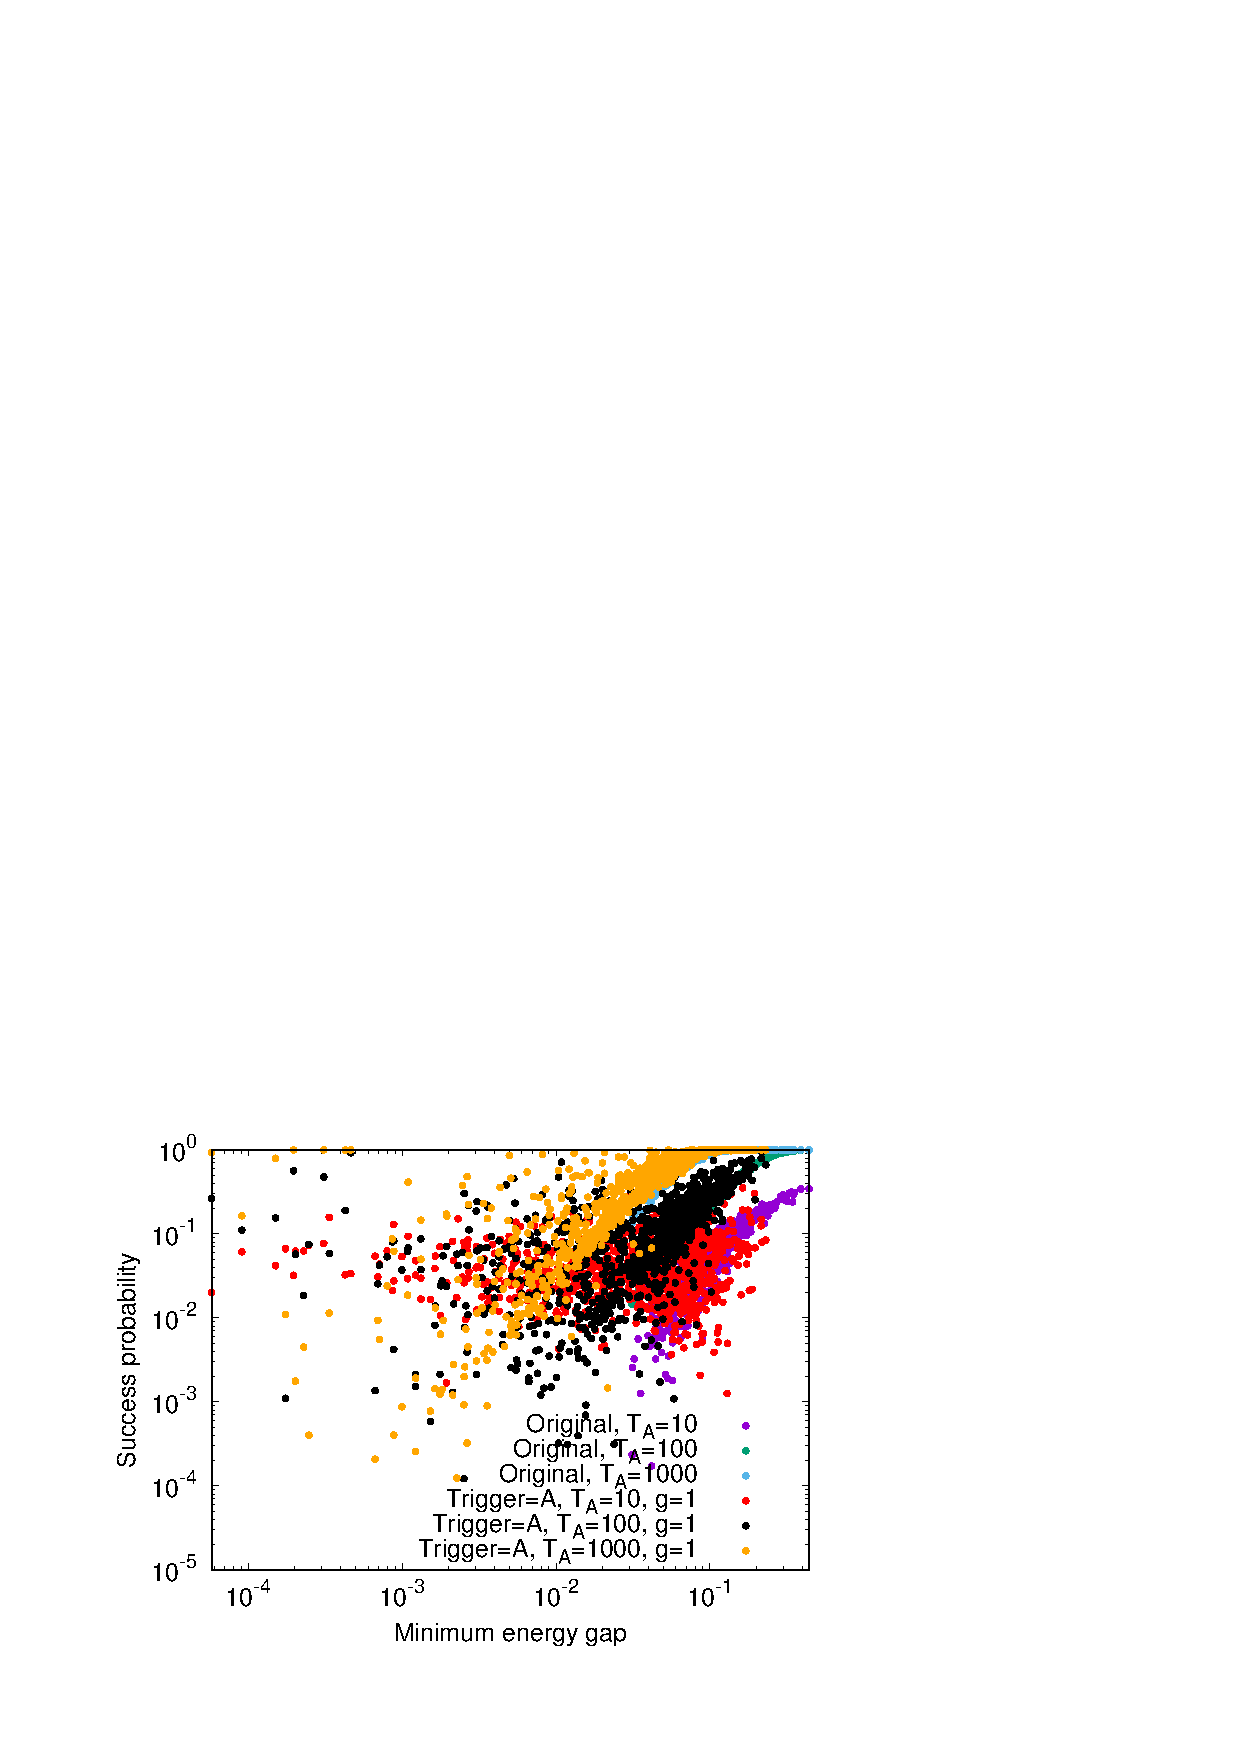
\includegraphics[scale=0.24]{SuccVsGap_OA_g1.png}
\caption{Success probability versus minimum energy plot for all the problems belonging to the set of 12-spin problems, for annealing times 10, 100 and 1000, in the absence and presence of the anti-ferromagnetic trigger.}
\label{fig:a36}
\end{figure}

It was observed that compared to the success probability Versus minimum energy gap corresponding to Hamiltonian where anti-ferromagnetic trigger is added with g=0.5 (see Fig. (\ref{fig:a17})), the scattering in case of adding the anti-ferromagnetic trigger with g=1 is larger for all the three annealing times. This indicates that the success probability is benefiting through non-adiabatic mechanisms for a larger fraction of problems in this case. One of the plausible reasons for which can be the increased number of energy anti-crossings between the ground state and the first excited state of the Hamiltonian. It can also be observed that unlike in Fig. (\ref{fig:a17}) the curves for this case can be more easily distinguished to roughly have the Landau-Zener form, and that points are not as restricted towards the left as a consequence of adding the trigger. This can thus be attributed to the presence of cases with enlarged minimum energy gaps as well.


\section*{g=2}
Finally, in this section the effects of adding the anti-ferromagnetic with strength 2 will be discussed.\\
Figs. (\ref{fig:a37}) and (\ref{fig:a38}) show the distribution of the relative success probability after adding the anti-ferromagnetic trigger for $T_A$=10 and $T_A$=100. In this case, only 1.5\% were found to have an improved success probability after adding the trigger for $T_A$=10. Upon increasing the annealing time to 100, this percentage increases to 15.8\%, and to 22.5\% for $T_A$=1000. This is in contrast with the observations from the previous sections where the percentage of the cases with improved success probability is the maximum for $T_A$=10. 

\begin{figure}[H]
\centering 
\includegraphics[scale=0.21]{A_T10_g2.png}
\caption{The distribution of relative success probability $\dfrac{p^A}{p^O}$ for $T_A$=10 and g=2. 1.5\% of the cases were found to have a higher success probability after adding the trigger.}
\label{fig:a37}
\end{figure}
\begin{figure}[H]
\centering 
\includegraphics[scale=0.21]{A_T100_g2.png}
\caption{The distribution of relative success probability $\dfrac{p^A}{p^O}$ for $T_A$=100 and g=2. 15.8\% of the cases were found to have a higher success probability after adding the trigger. }
\label{fig:a38}
\end{figure}
Furthermore, for $T_A$=1000 the spread of the relative success probability was only from 0.63 to 1.58, i.e. the effect of adding the trigger was only marginal. Additionally, for 44.8\% of the cases the relative success probability was found to be 1.

Fig. (\ref{fig:a39}) shows the scatter plot of the minimum energy gaps after adding the anti-ferromagnetic trigger ($\Delta^A$) with the original minimum energy gap ($\Delta^O$), for g=2. For this case it was observed that for 79.8\% of the problems the minimum energy gaps were reduced as a consequence of adding the trigger. It was also noticed that with the anti-ferromagnetic trigger of strength 2 the energy spectrum changed significantly in terms of the number of anti-crossings between the ground and the first energy level, and the proximity of the higher energy levels. As an estimate of the same, Tab. (\ref{tab:a5}) shows the percentage of cases with different number of anti-crossings.
\begin{table}[H]
\centering
\renewcommand{\arraystretch}{1.5}
\begin{tabular}{|c|c|}
\hline 
Number of anti-crossings & Number of cases (\%) \\ 
\hline 
1 & 0.1 \\ 
\hline 
2 & 13.2 \\ 
\hline 
3 & 43.9 \\ 
\hline 
4 & 36.3 \\ 
\hline 
5 & 6.5 \\
\hline
\end{tabular} 
\caption{Number of cases with different number of anti-crossings after adding the anti-ferromagnetic trigger with g=2.}
\label{tab:a5}

\end{table}
\begin{figure}[H]
\centering 
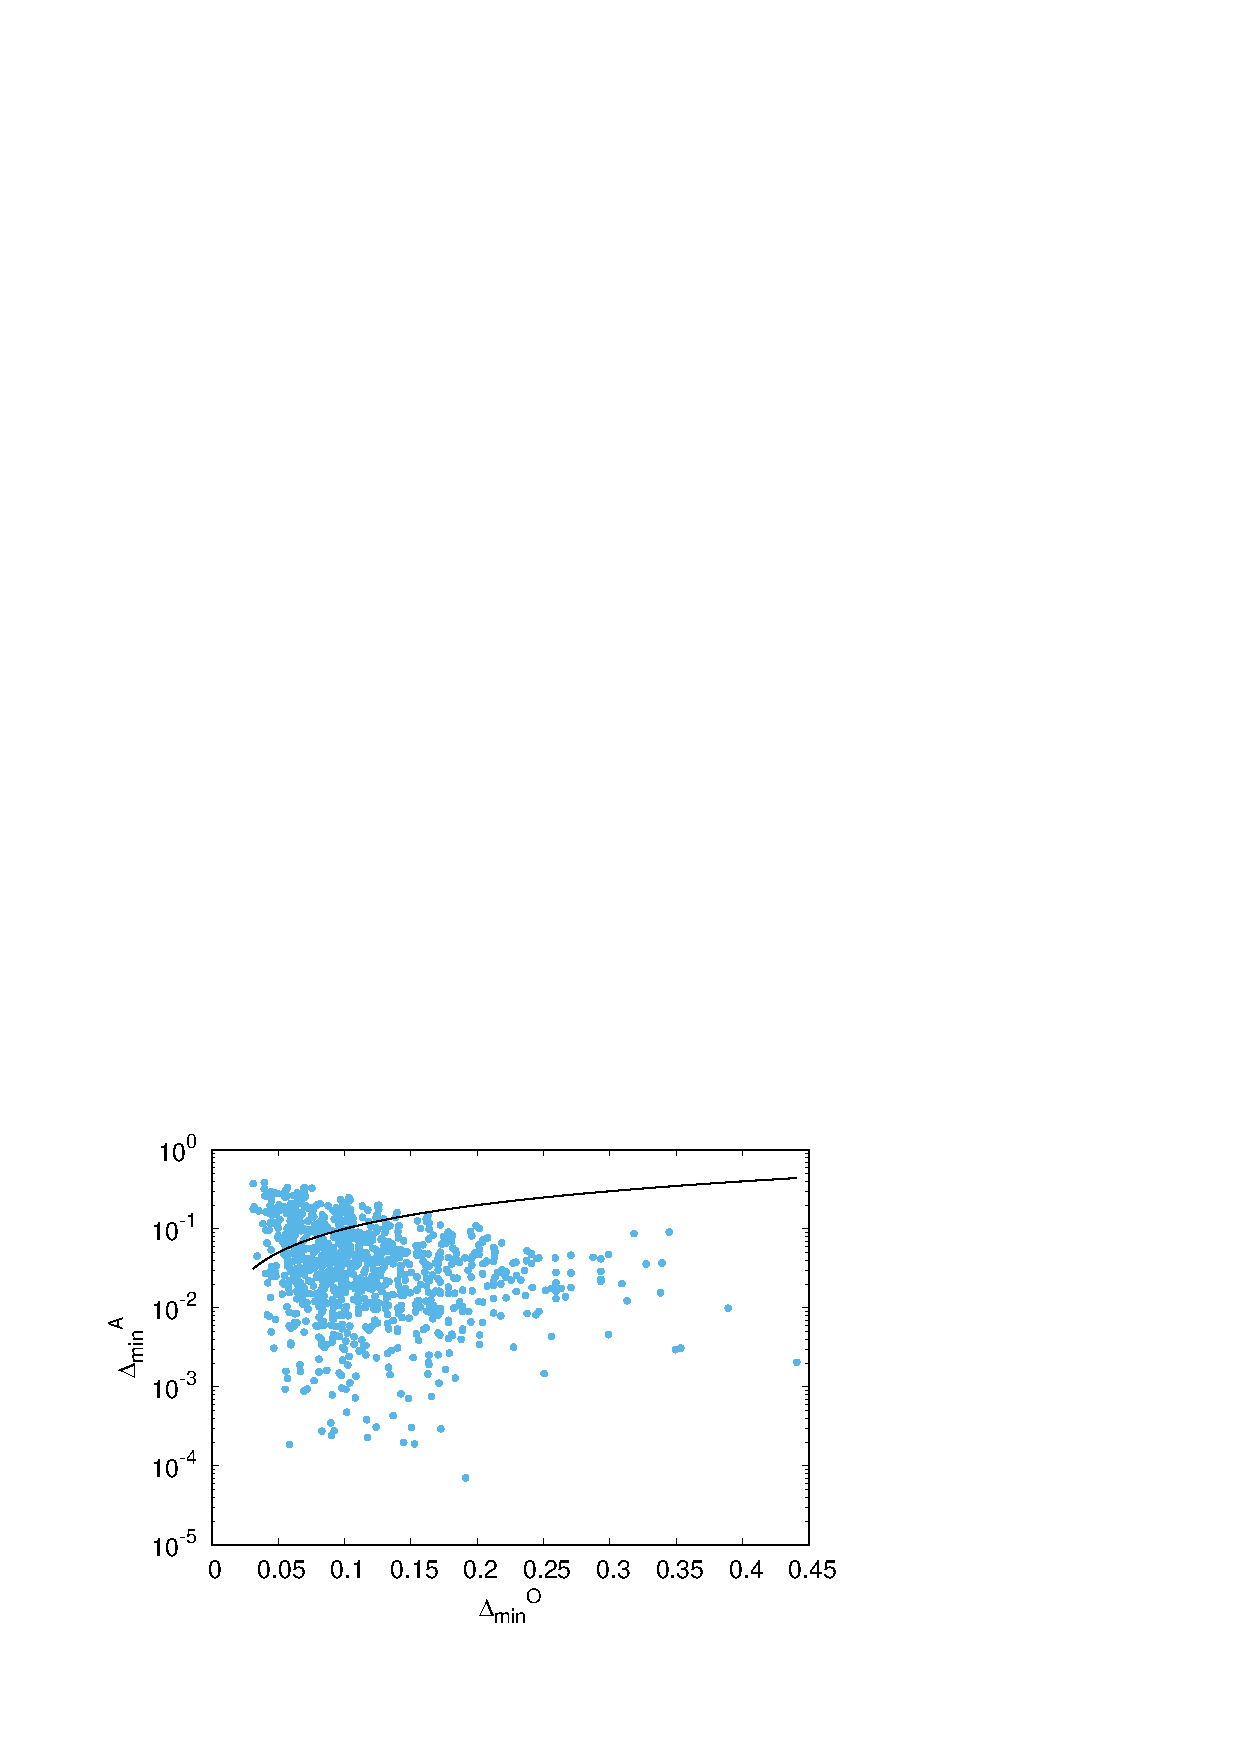
\includegraphics[scale=0.2]{MinGap_A_g2.png}
\caption{A plot of the minimum energy gaps after adding the anti-ferromagnetic trigger with g=1 ($\Delta_{min}^A$), with the original minimum energy gaps ($\Delta_{min}^O$). For 79.8\% of the minimum energy gap was found to have decreased after adding the trigger.}
\label{fig:a39}
\end{figure}

Next, to assess the difficulty of problems affected by adding the anti-ferromagnetic trigger to the Hamiltonian, Fig. (\ref{fig:a41}) shows the scatter plot of the success probability upon including the anti-ferromagnetic trigger ($p^A$) with that of the original Hamiltonian ($p^O$). 


\begin{figure}[H]
\centering 
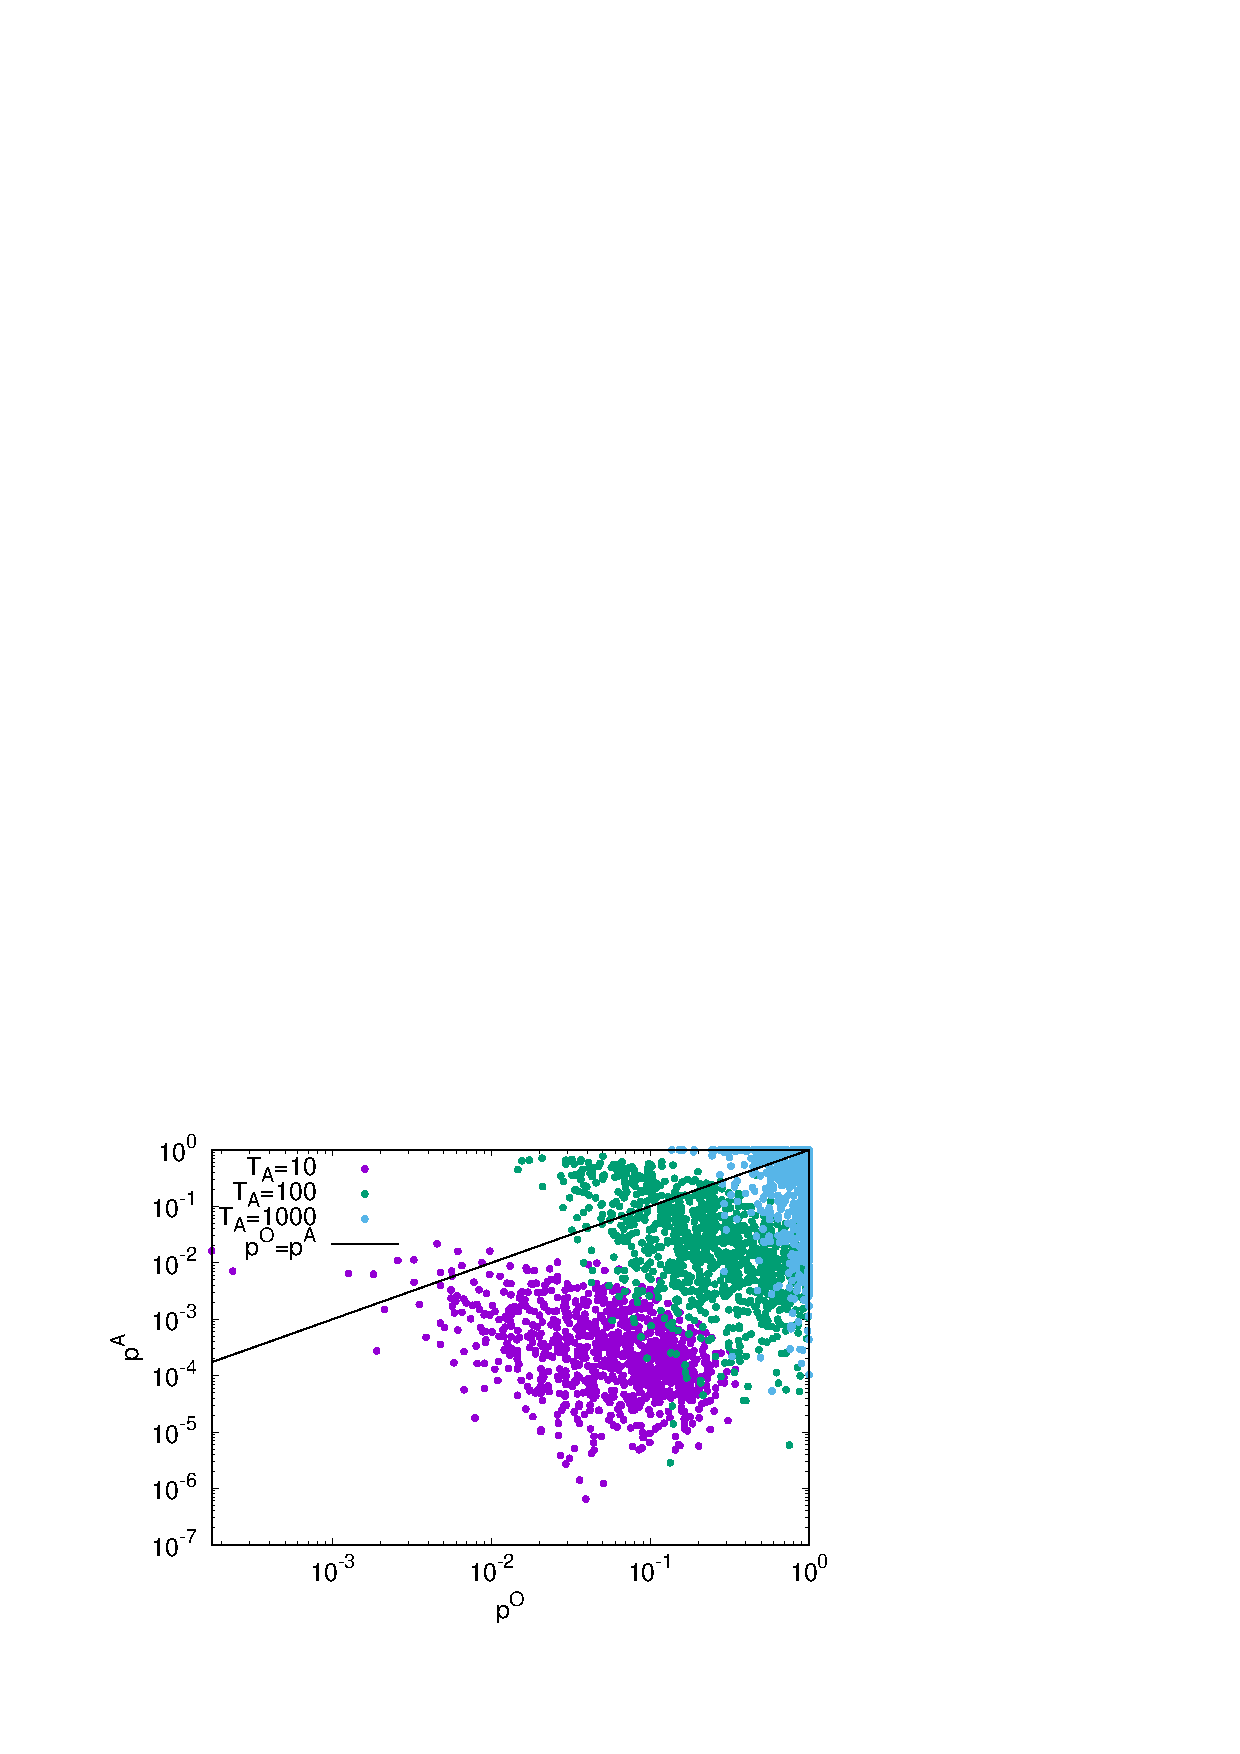
\includegraphics[scale=0.22]{ProbScat_g2.png}
\caption{A plot of the success probabilities after adding the anti-ferromagnetic trigger with g=2 ($p^A$), with the original success probabilities($p^O$) for annealing time 10, 100 and 1000.}
\label{fig:a40}
\end{figure}
In this case too, the spread of the problems improved by adding the trigger was the largest for annealing time of 10. This can be attributed to the small original success probability ($p^O$) for a small annealing time of $T_A$=10, or to the non-adiabatic evolution mechanisms leading to larger overlap with the ground state. For the cases with largest relative success ratio corresponding to $T_A$=10, having smaller original success probability was found to be the main reason for large improvements (maximum relative success ratio being 93.91). For $T_A$=100 and $T_A$=1000 the improvements become successively limited, with maximum relative success probabilities of 41.36 and 7.34 respectively. This is a consequence of increasing original success probabilities for longer annealing times. For understanding the mechanisms involved in the evolution of the state after adding the trigger, the scatter plots of the minimum energy gaps after adding the trigger ($\Delta^A$) against the original minimum energy gaps ($\Delta^O$) have been shown for the cases with improved success probability in Figs. (\ref{fig:a41}), (\ref{fig:a44}), and (\ref{fig:a45}) for annealing times of 10, 100 and 1000 respectively.\\


\begin{figure}[H]
\centering 
\includegraphics[scale=0.3]{selected_T10_g2.png}
\caption{For the cases with higher success probability for $T_A$=10 after adding the anti-ferromagnetic trigger with g=2, the scatter plot of minimum energy gaps $\Delta^A $ with $\Delta^O$. 3 out of 15 of such cases were found to have smaller minimum energy gaps after adding the trigger.}
\label{fig:a41}
\end{figure}

From Fig. (\ref{fig:a39}), it can be noted that 12 out of the 15 problems with improved success probability have larger minimum energy gaps upon including the anti-ferromagnetic trigger. Furthermore, all of these problems had a larger relative success probability for longer annealing times of 100 and 1000 as well. This suggests that adding the trigger widened the minimum energy gap enough for the evolution to become closer to adiabatic for $T_A$=10.\\

However, unlike the case in the previous sections, only 3 problems (problem number 478, 693 and 871) with improved success probability had a smaller minimum energy gap after adding the anti-ferromagnetic trigger. All these problems were benefited from the similar non-adiabatic evolution of the state. The energy spectrum and the instantaneous energy expectation values of the state for the original Hamiltonian and the Hamiltonian after adding the trigger have been shown in Fig. (\ref{fig:a42}) and (\ref{fig:a43}) for problem 693. For the original Hamiltonian, the state of the system shifts to the first excited state on approaching the energy anti-crossing, and closely follows it thereafter. This makes the overlap of the system state with the ground state negligible. However, in the case where the anti-ferromagnetic trigger is included, the minimum energy gap reduces, making it feasible for the state to transit to the higher excited levels. Consequently, the state ends in a superposition state consisting of higher energy levels, which coincidentally has a larger overlap with the ground state of the Hamiltonian.


\begin{figure}[H]
\centering 
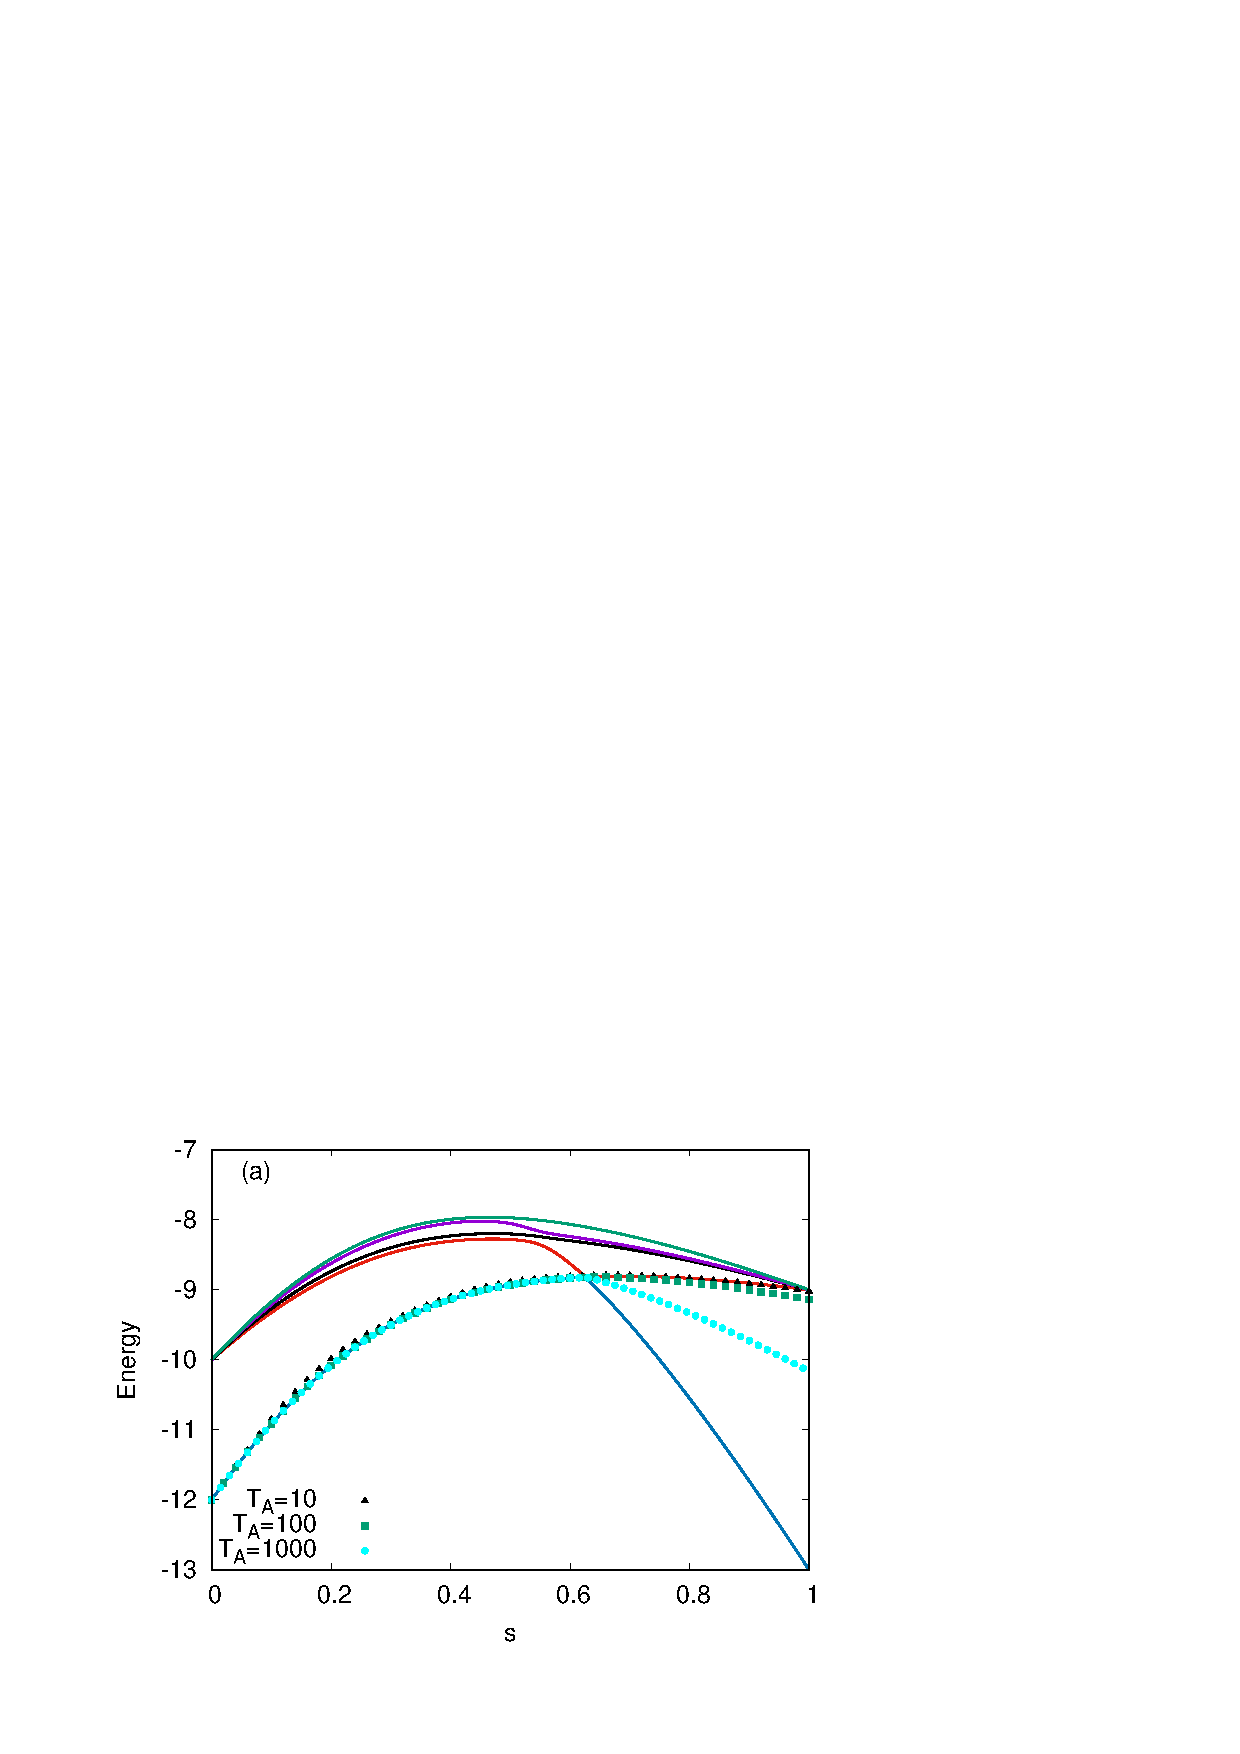
\includegraphics[scale=0.2]{693_O_g2.png}
\caption{Energy spectrum and instantaneous energy expectation values for the original Hamiltonian in problem 693.}
\label{fig:a42}
\end{figure}
\begin{figure}[H]
\centering 
\includegraphics[scale=0.2]{693_A_g2.png}
\caption{Energy spectrum and instantaneous energy expectation values of the state after adding the anti-ferromagnetic trigger to Hamiltonian in problem 693, after adding the anti-ferromagnetic trigger with g=2.}
\label{fig:a43}
\end{figure}

In this problem, the success probability reduces after adding the trigger for both $T_A$=100 and $T_A$=1000. For the spectrum with the trigger and $T_A$=100, the system state shifts to the first excited state at the first anti-crossing, from where it soon shifts to the higher excited states. Unlike the case for $T_A$=10, this time the state follows them closely, resulting in a vanishing overlap with the ground state. For $T_A$=1000, on the other hand, the state shifts to the first excited state only on reaching the second anti-crossing. Since the original minimum gap is larger for this problem, the original success probability is larger for this annealing time.

\begin{figure}[H]
\centering 
\includegraphics[scale=0.3]{selected_T100_g2.png}
\caption{For the cases with higher success probability for $T_A$=100 after adding the anti-ferromagnetic trigger with g=2, the scatter plot of energy gaps $\Delta^A $ with $\Delta^O$. 118 out of 158 of such cases were found to have larger minimum energy gaps after adding the trigger.}
\label{fig:a44}
\end{figure}

118 cases out of 158 cases found to have an improved success probability after adding the trigger, for $T_A$=100, also had a larger minimum energy gap as a result of adding the trigger. It was also noted that all of these cases also had a  relative success probability greater than 1 for $T_A$=1000. The energy spectra for 6 of the remaining 40 cases were studied to understand the evolution of the state, leading to an improve success probability. Same mechanics was found to be governing the dynamics of the state.
\begin{figure}[H]
\centering 
\includegraphics[scale=0.3]{selected_T1000_g2.png}
\caption{For the cases with higher success probability for $T_A$=1000 after adding the anti-ferromagnetic trigger with g=2, the scatter plot of energy gaps $\Delta^A $ with $\Delta^O$. 189 out of 225 of such cases were found to have larger minimum energy gaps after adding the trigger.}
\label{fig:a45}
\end{figure}
For $T_A$=1000, 189 out of 225 cases where the success probability after adding the trigger was noted to be larger than the original success probability were found to have a larger minimum energy gap after adding the trigger. The energy spectra for 4 of the rest 36 cases were also studied. Furthermore, 13 of these cases were also found to have larger success probability for $T_A$=100.


Finally, fig. (\ref{fig:a42}) shows the success probability versus minimum energy gap for all the problems of the set, for the original Hamiltonian, and the Hamiltonian after adding the trigger. 

\begin{figure}[H]
\centering 
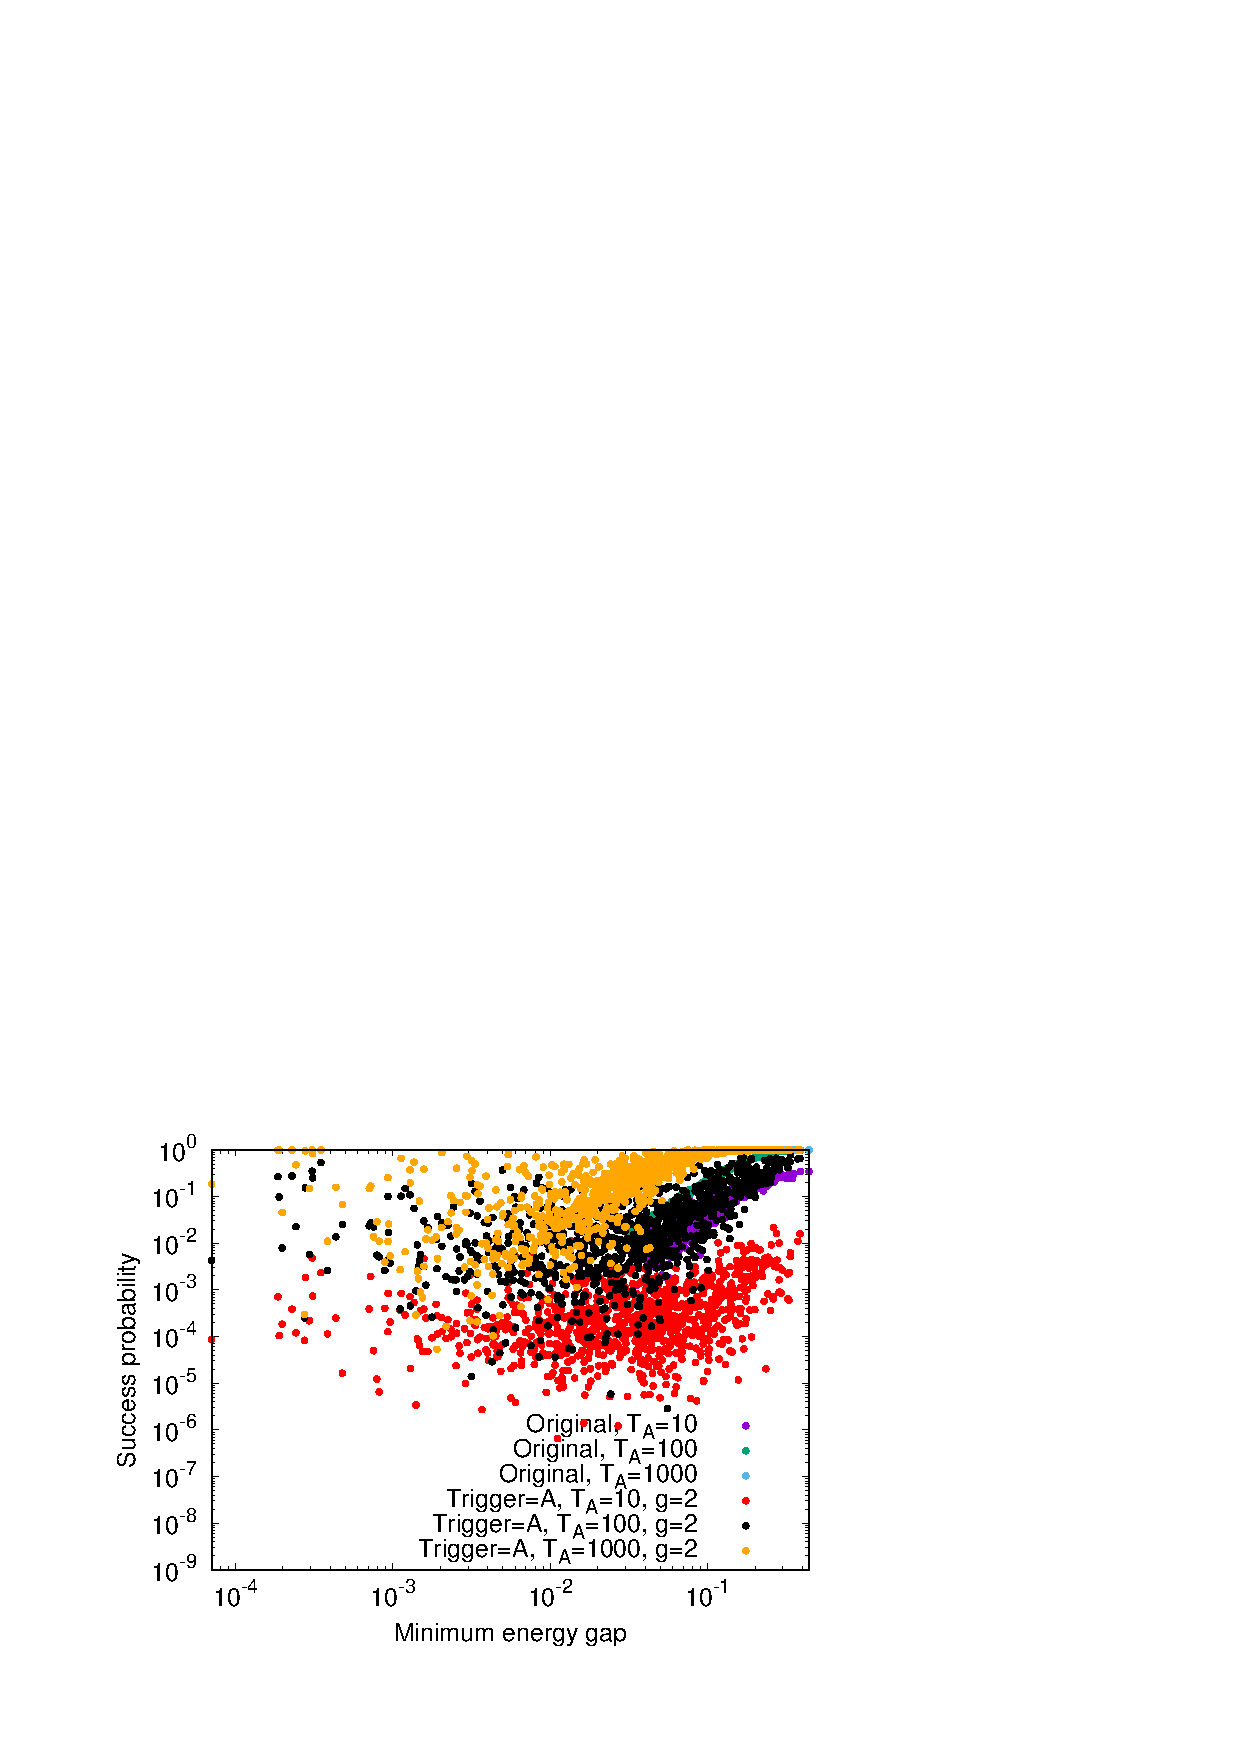
\includegraphics[scale=0.24]{SuccVsGap_OA_g2.png}
\caption{Success probability versus minimum energy plot for all the problems belonging to the set of 12-spin SAT problems, for annealing times 10, 100 an 1000, in the absence and presence of ferromagnetic trigger.}
\label{fig:a46}
\end{figure}

In this case, the scattering was found to have increased even more as compared to the case with g=1. This indicates that more problems deviated from the Landau-Zener formula in this case, suggesting a non-adiabatic evolution of the state in more number of problems.
\end{document}